\chapter{Реализация программного комплекса NA64}

Обработка данных установки требует преобразования
сигналов детекторов в согласованное представление в
рамках модели события и реконструкции физических величин
на их основе с применением калибровочной информации в
физические величины. Рассмотрим конкретные реализации
компонент программного комплекса выполняющего такую задачу
в рамках предложенной архитектурной концепции.

Так, многие элементарные варианты использования эффективно обобщаются
в рамках искусственных языков с заданной формальной грамматикой,
определяемой контекстом использования. В частности, они обеспечивают мощные
выразительные средства для повторяющихся задач:
выбор детекторов, запросы к модели события, описание калибровочных
данных.

Применение конкурирующих численных методов и их динамическая композиция
могут быть обобщены в рамках машины конечных состояний, которые применяются,
в частности, к задаче аппроксимации амплитудной функции сигналов калориметров
или реконструкции треков с проверкой конкурирующих гипотез.

Выбор форматов данных должен быть обоснован в рамках заданных
архитектурных инвариантов, фиксируя протоколы обмена данными между
основными компонентами.

\section{Предметно-ориентированные языки}

Для решения локальных задач возникающих в узкой предметной области,
часто прибегают к конструированию т.н. предметно-ориентированных
формальных языков~(англ. \emph{domain-specific languages}, также
<<проблемно-ориентированные языки
программирования>>, \acrshort{dsl})~\cite{DSL-Fowler2011}. Такие искусственные
языки не обязательно обладают качествами присущими языкам программирования
общего назначения: они могут не обладать полнотой по Тьюрингу (язык
запросов SQL в редакции 1992 года~\cite{ISO90751992}, язык
регулярных выражений~\cite{thompson1968programming},
не иметь выразительных средств для арифметических операций или операций со
строками, абстракциями ввода-вывода и т.п. Взамен такие языки
предоставляют специализированные выразительные средства для решения узкого
класса прикладных задач посредством более компактных нотаций.

В качестве примеров таких языков в \acrshort{hep} можно привести
математическую нотацию численных функций и логических предикатов
<<TFormula>> программного окружения ROOT \cite{ROOT-framework} или язык численных
функций встраиваемый в интерпретатор GDML в~\cite{Berra2011Geant4SO}.

Создание программных инструментов для интерпретации \acrshort{dsl}
возможно при помощи автоматизированных средств, на основе
формализованной специальным образом грамматики~\cite{alfred2007compilers}.
Средства вводят следующие ограничения на уровнях лексического
разбора~(\emph{lexer}) и семантического анализатора~(\emph{parser}):
\begin{itemize}
    \item Лексический интерпретатор поддерживает регулярные
    грамматики (тип 3 по иерархии Хомского~\cite{chomsky1956three}),
    т.е. эквивалентные детерминированному конечному автомату. Такие грамматики
    позволяют право- или леворекуррентные определения правил, однако
    не их сочетания.
    \item Парсер поддерживает более узкий набор грамматик  LALR(1)
    (\emph{look-ahead, left-to-right}, тип 2 по иерархии Хомского) ---
    анализатор с ограниченным односимвольным упреждением на основе
    левостороннего восходящего разбора.
\end{itemize}
Эти ограничения позволяют конструировать довольно сложные
грамматики, вполне достаточные для реализации небольших \acrshort{dsl},
не требующих полной выразительной мощности контекстно-свободных
грамматик и не содержащих конструкций с неоднозначным синтаксисом
или контекстно-зависимыми правилами.
%, что актуально в языках программирования общего назначения.

Формальные описания грамматик языков и программ реализующих
примитивы исполнения вынесены в приложение~\ref{appendix:dsl-grammars}.

\subsection{Числовой идентификатор детектора и язык селекторов}

Одним из частых предусматриваемых обобщающих сценариев использования
конвейерного шаблона проектирования является применение отдельного
обработчика к выборке объектов по ключу (идентификатору детектора)
в коллекции объектов. Например, в задачах анализа и
онлайн-диагностики детектора
нужно построить гистограмму величины ассоциированной с конкретным
детектором. В другом случае -- назначить различные обработчики
разным группам детекторов. В этих случаях целесообразно предусмотреть гибкий
механизм определения подмножества посредством специализрованных
выражений.

В подобных случаях нередко прибегают к индексированию детекторов и связанных
с ними данных посредством строковых идентификаторов. Так например, в системе
сбора данных COMPASS и NA64 внутренняя номенклатура идентификаторов детекторов
построена в соответствии со следующей грамматикой (здесь и далее
грамматики формулируются в форме
Бэкуса-Наура~\cite{backusNaurAlgol1963revised}):

\begin{verbatim}
    det ID ::= <detector kin> <station number>
    
    detector kin ::= <буква> | <detector kin> <буква>
    
    station number ::= <цифра> | <station number> <цифра>
\end{verbatim}
где \texttt{<буква>} и \texttt{<цифра>} --- терминалы грамматики.

Примерами грамматически корректных имён детекторов в такой простейшей
грамматике являются \texttt{ECAL0} (калориметр ECAL), \texttt{HCAL3}
(третий модуль адронного калориметра), \texttt{MM03} и т.д.

Тогда выборку детекторов можно произвести на основе
какого-нибудь \acrshort{dsl} предназначенного для поиска строкового
соответствия -- например языка регулярных выражений или
языка поисковых шаблонов Unix~(\emph{wildcard}~\cite{wildcards-mcilroy1987research}).

На практике, эта грамматика в эксперименте COMPASS носит лишь
рекомендательный характер. Сложные станции этого спектрометра, состоящие из
нескольких координатно-чувствительных плоскостей (зон, в поперечном
сечении) обуславливают необходимость более тонкого деления. Так, по мере
развития эксперимента COMPASS в номенклатуру его детекторов
оказались введены такие элементы как \texttt{ST03ub}, \texttt{MA01c},
\texttt{MP03MX1}, вовсе не следующие формальным правилам общим более чем
для единственной станции. Выбор станции или плоскости всё ещё можно
реализовать при помощи строковых \acrshort{dsl} -- то есть, с одной стороны это
довольно гибкий подход.

С другой стороны, во-первых, отсутствие формальной грамматики приводит
к неоднозначности при выборе отдельных чувствительных элементов,
затрудняет выбор связанных с ними транзитивно (в рамках модели
события) экземпляров данных.
% нужны ли тут примеры? что если я хочу выбрать только стриповые части
% микромег без пиксельных частей?
Во-вторых, операции строкового сравнения в общем случае менее
эффективны, чем сравнение числовых идентификаторов. С учётом того,
насколько часты на практике такие запросы к объектной
модели (поиск по ключу, различные условия выборки и фильтрации),
целесообразно предусмотреть программное средство для биективного
преобразования строковых и числовых идентификаторов для перечисления
номенклатуры детекторов. При этом всё ещё возможно предусмотреть
определённую свободу в именовании, часто диктуемую ситуативным
удобством при размещении детекторов на пучке и подключении
электроники.

Большим преимуществом числовых идентификаторов является удобство
их использования в ассоциативных контейнерах на основе бинарных
деревьев поиска (в частности, красно-чёрных деревьях реализованных
в библиотеке шаблонов STL C++). Это позволяет существенно упростить
работу с объектной моделью события в C++, снабдить порядок
итерирования дополнительной семантикой, обеспечить эффективный
компромисс между быстродействием при прямых запросах по ключу
и использованием памяти. Обращения к такому контейнеру не подразумевают
вычисления хеш-сумм, символьных сравнений и др. Поиск по ключу имеет
сложность $O(\text{log}~n)$.

%В дальнейшем, в рамках работы будем ссылаться на язык и его реализацию
%его интерпретатора по имени
%<<DSuL>> (\emph{detector selection micro-language}).

\subsection{Язык запросов модели события}

Объектная модель события снабжённая рефлексией сама по себе
уже позволяет строить обобщённые обработчики в рамках конвейерного
шаблона проектирования.

Так, например, достаточно определить класс обработчика строящего
одномерную гистограмму случайной величины, параметризуемый
идентификатором ссылающимся на определённый числовой атрибут события,
чтобы реализовать возможность построения всех одномерных гистограмм
любого атрибута в событии. Таким образом, введение новых атрибутов
посредством выведения шаблонов не требует никаких дополнительных
операций со стороны разработчика для создания гистограмм вводимых новым
типом значений.

В качестве идентификатора атрибута можно использовать нотацию близкую
к принятой в C++: например, выражения \texttt{SADCHits.time} или
\texttt{APVClusters.hits.x} достаточно близки к нотации разыменования
атрибутов в C++.
%Тем не менее, такая запись во втором случае допускает
%различие в интерпретации -- неясно, какая из двух коллекций (\texttt{APVClusters}
%или \texttt{APVClusters.hits}) должна итерироваться первой.

Помимо этого, нередки случаи, когда необходимо выполнить некоторые (элементарные)
преобразования с полями события, или применить фильтрацию на уровне
атрибута с типом-коллекцией. % так, как это определено, например, в DSuL.

С этой целью в программном окружении предусмотрена интеграция с
\acrshort{dsl} предназначенным для работы с потоками организованных
иерархически
объектов с заранее известной схемой (топологией). Он поддерживает базовые
операции фильтрации и арифметики значений, однако не позволяет изменять
топологию данных (что является одним из сознательных ограничений по сравнению с
более универсальными \acrshort{dsl}, такими как SQL или GraphQL \cite{graphql-comparative}).

Основными вариантами использования языка являются:
\begin{itemize}
    \item Задание логических условий для дискриминации событий или элементов
    коллекций внутри события (таких, как кластеры или треки).
    \item Задание генераторных выражений для построения N-мерных гистограмм.
    \item Задание генераторных выражений для представления данных физических
    событий в табличном виде.
\end{itemize}
Во всех случаях, язык должен допускать арифметические вычисления,
определение новых элементов объектной модели (существующих в рамках
запроса), применение агрегатных функций над выборками.

\subsection{Описание калибровочных данных}

%В экспериментальной физике нередко возникает необходимость представления
%информации с хронологической привязкой к астрономическому времени, либо
%в соответствии с внутренней хронологической номенклатурой (например, к
%периодам набора статистики, когда конфигурация установки в достаточной степени
%неизменной). Источником таких данных могут быть как внешние измерения:
%результаты геодезической съёмки, обеспечивающие относительную геометрическую
%привязку детекторов, сведения о температуре, влажности и давлении в
%экспериментальном зале, значения токов газовых смесей в рабочих объёмах
%установки и т.д. К тому же классу относятся и данные, регистрируемые
%непосредственно подсистемами детекторов: коэффициенты масштабных
%преобразований (амплитудных и временных), пороговые значения для
%подавления фона и шумов, а также коэффициенты, определяющие шкалы
%преобразований для различных типов аналого-цифровых и цифровых
%преобразователей. В дальнейшем под калибровочной информацией будем
%понимать весь объём данных, не относящихся непосредственно к
%экспериментальной статистике, но требующих временной привязки и
%используемых в алгоритмах обработки и реконструкции.
%
%В общем случае задача управления таким набором данных, подразумевающая
%прежде всего быструю операцию поиска по хронологическому ключу, и, с
%меньшим приоритетом, -- операции вставки и удаления записей, решается при
%помощи реляционных таблиц организованных под управлением различных СУБД.
%
%При этом задача интеграции СУБД с программами обработки, в особенности
%на ранних этапах разработки и прототипирования, нередко представляет
%определённую техническую сложность из-за необходимости сопровождения
%участков программы отвечающих за преобразование табличных данных в массивы
%записей (экземпляры объектной модели), разрешение коллизий, сопряжение
%информации из различных таблиц.
%
%С целью упростить процедуру ранней разработки и предоставить инструмент
%облегчающий дальнейший перенос калибровочной информации под управление
%СУБД, было разработано программное решение опирающееся на представление
%калибровочной информации в виде текстовых таблиц.
В общем, под \emph{калибровочной информацией} в данной работе понимается
совокупность данных, не относящихся непосредственно к событиям, но
требующих временной привязки и необходимых для алгоритмов обработки и
реконструкции. К такому классу относятся, например, результаты геодезических
измерений, обеспечивающие относительное позиционирование детекторов,
сведения о внешних условиях (температура, влажность, давление, параметры
газовых смесей), а также коэффициенты и пороговые значения, определяемые
по показаниям самих детекторов и задающие шкалы преобразования
измерительных каналов.

Управление калибровочной информацией сводится главным образом к
задаче быстрого поиска по временным ключам при поддержке операций
вставки и удаления записей. Традиционно она решается с
использованием реляционных таблиц под управлением \acrshort{dbms}.
Однако на стадии прототипирования интеграция с \acrshort{dbms}
может быть затруднена необходимостью преобразования табличных структур в объекты,
согласования информации из разных таблиц и обработки коллизий.

С целью упростить эти процедуры на ранних этапах разработки и
обеспечить возможность последующего переноса данных в полноценные
\acrshort{dbms} было реализовано программное решение, основанное на
представлении калибровочной информации в виде текстовых таблиц.
%Программное решение представлено библиотекой шаблонных процедур,
%работающих с индексом временных интервалов которым в соответствие
%поставлены записи состоящие из идентификатора артефакта и типа
%данных.
Решение предоставляется в виде библиотеки шаблонных
процедур, работающих с индексом временных интервалов. Интервалам
в индексе сопоставляются записи, включающие идентификатор
артефакта-источника и соответствующий тип данных.

%Индекс представляет собой шаблонный класс
%параметризуемый произвольным типом ключа для которого посредством
%шаблонной специализации C++ задаются операция сравнения и нулевой
%элемент соответствующий открытому интервалу.
Индекс построен как шаблонный класс, параметризуемый произвольным
типом ключа. Для этого ключа посредством специализации шаблонного
класса C++ задаётся единственная операции сравнения, а также определяется
нулевой элемент, интерпретируемый как открытый интервал.

Библиотека предоставляет реализации процедур для рекурсивного
разбора текстовых файлов с табличной информацией и преобразования
её в пользовательские типы данных (посредством шаблонной
специализации). Подразумевается, что документы помимо таблиц могут
содержать разметку (метаданные) влияющую на
лексическое преобразование. Так важным практическим вариантом
использования  является переопределение отдельных элементов для
временных подинтервалов, определение неполных данных, фрагментация
таблиц с целью более гибкой настройки логики применения данных,
поддержка арифметических преобразований (встроенный интерпретатор
формул) и т.д.
Библиотека содержит средства для рекурсивного разбора текстовых файлов
с табличными данными и их преобразования в пользовательские типы
(через механизмы статического полиморфизма). Предполагается,
что документы могут включать не только таблицы, но и метаданные,
аннотирующие калибровочную информацию и влияющие на процесс
лексического анализа. На практике это позволяет реализовывать
такие сценарии, как переопределение отдельных элементов для
временных подинтервалов, задание неполных данных, фрагментация
таблиц.

Лексический разбор документов организован на основе регулярных
выражений с настраиваемой грамматикой, которая описывает
искусственный язык разметки, подобный
языку описания гипертекстовых документов HTML~\cite{berners1989information},
языку спецификации каскадных стилевых таблиц CSS~\cite{lie1996cascading}),
или языку конфигурационных файлов~\cite{yaml-rfc9512}.
Лексический разбор также включает интерпретатор
арифметических выражений для выполнения арифметических
преобразований (\texttt{TFormula}~\cite{ROOT-framework}).
Пользовательский код
может изменять разделители табличной разметки, способы
интерпретации и маркеры метаданных, учитывать информацию
о путях размещения артефактов.

Решение оптимизировано под цикл разработки подразумевающий
управление калибровочными данными посредством размещения их
в файлах. На финальной стадии синхронизация с \acrshort{sw}
производится сетевым сервисом настроенным на автоматическое
отслеживание сетевого ресурса на котором публикуются документы.

%В заключении нужно отметить, что хотя преобразование таблиц на этапе
%индексации артефактов не выполняется (таблицы интерпретируются только при запросе
%по ключу), необходимость построения индекса является
%естественным ограничением такой архитектуры.
Следует отметить, что преобразование таблиц в процессе индексации
не выполняется: они интерпретируются лишь при обращении по ключу.
Это обеспечивает гибкость, однако сама необходимость построения
индекса выступает архитектурным ограничением предложенного подхода.
\section{Динамические машины состояний}

Для решения задач выбора конкурирующих гипотез -- таких, как разделение
амплитудных импульсов во времени или выбор между гипотезами о
треке частицы,
%в рамках подхода быстрого прототипирования,
целесообразно прибегнуть к высокому уровню общности,
поскольку по мере появления новых детекторов и считывающей аппаратуры,
тестирования и разработки новых методов реконструкции сигналов,
необходимо производить исследование поведения существующих алгоритмов,
производить оптимизацию параметров и часто изменять систему.

Истинная функция отклика подвержена влиянию многих факторов: существенно
зависит от считывающей аппаратуры и изменяется в зависимости от вещества
рабочего объёма детектора.
%Используемая в качестве приближения
%\emph{модельная функция} $f(t,\vec{p})$ --- аппроксимация амплитуды в момент
%времени $t$ праметризуемая параметрами $\vec{p}$
С некоторыми допущениями, для реконструкции
можно применять упрощённую модель или быстрый алгоритм реконструкции с
потерей точности там, где ошибки не так важны как средняя картина
наблюдаемых распределений.

Например, при
мониторировании детекторов во время набора данных.
Напротив, для задач анализа целесообразно
стремиться к наиболее правдоподобной модели -- например, для улучшения
разрешения при реконструкции ливней в калориметрах, поскольку
малые амплитуды на периферии ливня приобретают большое значение
в дискриминационных логических схемах.

%Важно отметить, что помимо задачи
%разрешения откликов САЦП, общая постановка задачи справедлива и для
%задачи реконструкции треков, которая в общем формулируется чаще всего
Другим примером является реконструкция треков, сформулированная
как задача минимизации функционала статистики
$\chi^2$ % = \sum\limits_i (f((t_i,\vec{p}) - r_i)/\sigma_i)^2$
от некоторой (в общем -- нелинейной, необязательно аналитической)
функции параметризации
трека $f(t,\vec{p})$ по отношению к выбранным наборам показаний
координатно-чувствительных детекторов $\vec{r}_i$. При этом
%, как правило, при больших загрузках детекторов,
%типичных для современных экспериментов с большой светимостью,
для разрешения возникающих неоднозначностей применяются различные
алгоритмы отбора: в рамках общей задачи поиска трека~(англ. \emph{track finding})
поиск может производиться по известным пространственным
шаблонам~(англ. \emph{pre-patterning}),
на основе пространственных биекций,
разбиения на KD-дерево, и т.д. ~\cite{MankelTracking, artificial-retina-tracking-lhc}
Такие алгоритмы обычно дают довольно грубое
приближение для более высокоуровневого алгоритма аппроксимации трека,
существенно снижающее набор входных значений по отношению к прямому
комбинаторному перебору.

\subsection{Варианты использования}

Пусть \emph{модель} --- математическая
функция $f(x,\vec{p})$, определённая в зависимости от некоторого
аргумента $x_i$ и вектора параметров $\vec{p}$. Целью
\emph{процедуры минимизации} является отыскание таких параметров $\vec{p}$
при которых достигается наилучшее соответствие набору входных данных $y_i$
согласно некоторой метрике (реализация принципа максимального правдоподобия).
При этом под отдельной программной процедурой далее понимается
формализованный алгоритм осуществляющий преобразование вектора параметров
модели~$P(\vec{p}_a) = \vec{p}_b$ (т.е. не обязательно минимизация).
%Символически, можно записать, что для некоторой метрики $\mathbb{M}$
%преобразование заданное процедурой $P$
%т.е. целью процедуры как преобразования $P[\vec{p}_a] \rightarrow \vec{p}_b$
%является отыскание таких $\vec{p}_b$ при которых достигается
%условие~$\text{min}()$

Индуктивно выделяются как минимум следующие основные варианты
использования системы, с точки зрения пользовательского кода,
расширяющие исходный сценарий применения процедуры к
программной модели:
\begin{itemize}
    \item Выбор и \emph{установка начальных значений} параметров $\vec{p}$
    на основе исходной выборки значений $x_i$. Этот вариант
    подразумевает предварительное вычисление начальных приближений
    на основе широкого набора параметров регулирующих поведение
    поисковых алгоритмов.
    \item \emph{Применение алгоритма численной минимизации}. Помимо
    \acrshort{lms} сюда относится, например, фильтр Калмана в его
    различных модификациях,
    и в целом задачи линейного программирования допускающие выражение
    в виде линейно-алгебраических операций над модельной функцией с
    фиксированным набором параметров.
    \item Элементарный вариант использования состоит в прямом
    \emph{изменении параметров модельной функции}. Такой этап может быть
    полезен, например, при искусственном введении возмущения в
    линейных алгоритмах минимизации с целью преодоления локальных
    минимумов.
    \item \emph{Применение процедур к отдельным элементам} и подразумеваемая
    в таком случае \emph{декомпозиция модели} может понадобиться,
    когда с точки зрения численной процедуры минимизации, модель может
    быть тем или иным образом разложена (факторизована) на набор более
    элементарных независимых моделей, к каждой из которых необходимо
    применить определённый набор процедур. Например: аппроксимация
    функции отклика для значительно разнесённых во времени пиков,
    аппроксимация трека частицы на линейных участках в отсутствии
    магнитного поля, и т.д.
    \item Для \emph{сопоставления результатов} аппроксимации между
    конкурентными методами посредством определённой метрики (в частности,
    выбор наилучшей гипотезы о треке на основании $\chi^2$), необходима
    соответствующая формализация, делегирующая выполнение
    конкретной реализации компаратора.
    \item В тех случаях, когда метрика не может быть определена для
    моделей, и основным результатом является логическое условие применимости
    процедуры, целесообразно выделить вариант использования перебирающий
    процедуры до тех пор, пока очередной вариант не будет
    выполнен успешно (\emph{выбор подходящей модели}).
    \item Наконец, \emph{выбор или замена модельной функции} в рамках
    такого уровня общности тоже представляет собой вариант использования.
\end{itemize}

\begin{figure}
    \centering
    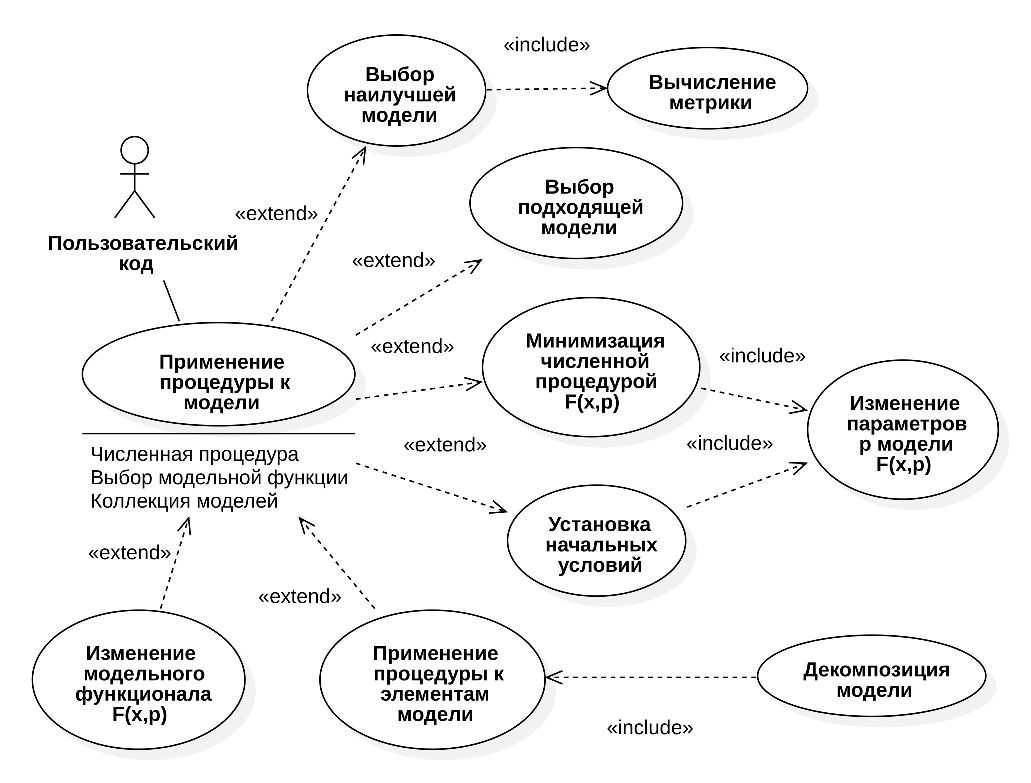
\includegraphics[width=0.95\linewidth]{images/umff-usecase-diagram-02.eps}
    \caption{Диаграмма вариантов использования программной библиотеки для
    решения задач численной минимизации с расширенной логикой (ветвление,
    сопоставление, перебор).}
    \label{fig:umff-usecases}
\end{figure}

Рисунок \ref{fig:umff-usecases} иллюстрирует отношения между перечисленными вариантами
использования.

\subsection{Компоненты машины конечных состояний}

Описанная структура вариантов использования подразумевает наличие по крайней мере
следующих элементов обобщённого поведения:
\begin{itemize}
    \item Составная процедура содержащая набор более простых процедур,
    делегирующая выполнение этому набору, и завершающаяся результатом
    отобранным согласно некоторому правилу (\emph{competing}).
    \item Составная процедура осуществляющая декомпозицию модели в тех случаях,
    когда модель это позволяет, инкапсулирующая набор более простых процедур,
    и применяющая этот набор по отдельности к каждому элементу
    декомпозиции~(\emph{breakdown}).
    \item Последовательность процедур в которой последующая применяется только
    в том случае, если текущая завершилась не успешно
    (\emph{fallback}).
    %Рисунок \ref{fig:fallback-example} содержит
    %пример машины конечных состояний, в которой применение процедуры
    %делегируется, а валидация выполняется самим элементом.
\end{itemize}

Этот базовый набор логических элементов позволяет конструировать сложные
условные последовательности, которые наиболее просто представить в виде
машин конечных состояний. В таких машинах состояниям отвечает
модель~($m_i:=f(x_i,\vec{p})$),
а переходам соответствует процедура~$P(\vec{p}_a) = \vec{p_b}$.

Техническое описание и спецификации вынесены в приложение~\ref{appendix:fsm-machine-prog}.

\subsection{Восстановление амплитудных сигналов}

На рисунке~\ref{fig:sadc-wf-fitting-example} приведён пример
восстановленного отклика ячейки электромагнитного калориметра от двух
импульсов слабо (не более чем на ширину) разнесённых во времени.
Пунктирной линией с коротким штрихом
изображён график конечно-разностной аппроксимации первой производной
по точкам сигнала, сплошными серыми линиями изображён результат
подгонки -- для отдельных импульсов и их восстановленная сумма.
Пунктирная линия с длинным штрихом отвечает начальным условиям.
%время в наносекундах против амплитуды в относительных единицах

\begin{figure}[ht]
    \centering
    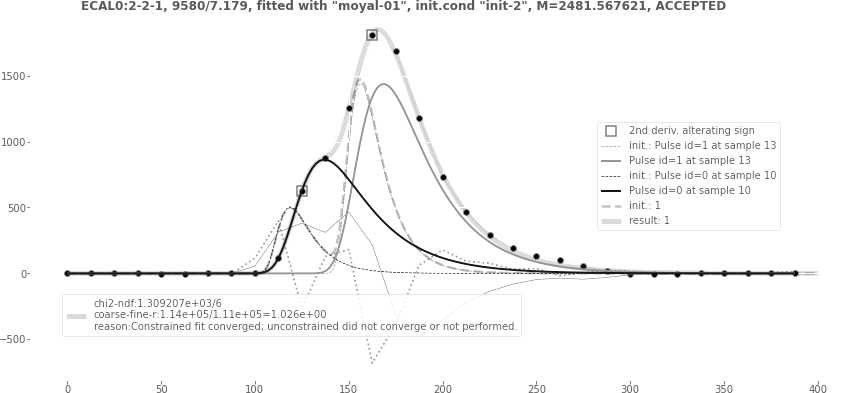
\includegraphics[width=0.99\linewidth]{images//illustrative/waveform-fit-result-example.png}
    \caption{Пример восстановления сигнала от двух частиц с малой временным
    интервалом}
    \label{fig:sadc-wf-fitting-example}
\end{figure}

Этот случай имеет большое значение в отношении физической картины,
поскольку подобную сигнатуру часто дают мюоны от
распадающихся в голове канала
пионов $\pi^{\pm} \rightarrow \mu^{\pm} \nu_\mu$ 
и каонов $K^{\pm} \rightarrow \mu^{\pm} \nu_\mu$,
или мюонные пары от реакций $\gamma Z \rightarrow Z \mu^{+}\mu^{-}$.

Наивный алгоритм построенный на выделении абсолютного максимума
не способен обнаружить первый импульс от слабоэнергетической частицы,
поскольку первый импульс вообще не даёт максимума. 

Второй пик распознаётся алгоритмом отыскания
импульсов, опирающимся на сигнатуру чередования роста и спада
функции. Аппроксимация моделью затем производится с учётом
индивидуальных особенностей ячейки, поскольку в общем случае
подгонка параметров модели в данной картине допускает неоднозначность
результатов. Кроме того, из-за присутствующей неоднозначности
весьма вероятна сходимость процедуры подгонки к локальному минимуму,
что решается посредством одновременного рассмотрения
нескольких конкурирующих гипотез (competing).

\section{Восстановление треков частиц}

Трекинг в NA64 необходим для определения энергии и идентификации
типа частиц попадающих в электромагнитный калориметр или
покидающих его. Важной особенностью экспериментов на фиксированной мишени
упрощающей рассмотрение треков частиц является допущение о
прямолинейности истинных траекторий частиц в отсутствии магнитного
поля и плотного вещества. Так в постановке для изучения электромагнитных
ливней инициированных электроном трекер
представляет собой двухплечевой спектрометр составленный
из нескольких газовых детекторов, расположенных по оси пучка с
условно-прямолинейными участками траектории до и после магнита,
перед массивным электромагнитным калориметром.
%с совокупным \emph{вкладом ??}.
Для мюонной постановки трекер дополнительно оснащается станциями
BMS (англ. \emph{beam momentum station}) в голове канала.
После калориметра устанавливается дополнительный
спектрометр представленный отклоняющим дипольным магнитом и дополнительными
станциями MicroMega и Straw с увеличенным
угловым аксептансом для идентификации частиц покидающих ECAL.

В целом, высокое пространственное разрешение
и сравнительно слабая оснащённость детекторами (по две или три станции на плечо,
выбранная, с тем чтобы минимизировать ионизационные потери и рассеяние), а
так же применение детекторов с гальванически связанными каналами (MicroMega)
обуславливают важные частные особенности трекера~NA64:
\begin{enumerate}
    \item Низкая заселённость за исключением второго спектрометра в мюонной
    постановке. В постановке с электронным или адронным пучком среднее
    число треков на событие -- $1{,}4$.
    \item Линейная протяжённость в десятки метров при сравнительно малой площади
    чувствительной поверхности детекторов в сотню $\text{см}^2$.
    \item Присутствие ложных срабатываний в MicroMega из-за гальванического
    соединения анодных полос (коммутации в одну сигнальную линию).
\end{enumerate}

С одной стороны эти особенности создают существенные методические
ограничения: невозможность эффективно использовать гало пучка для
выравнивания, и невозможность эффективно покрыть трекер в голове
канала расфокусированным пучком
для выравнивания и изучения эффективности трекера.

С другой стороны, при сравнительно высоком пространственном разрешении
трекера, дающим энергетическое разрешение не хуже $1~\text{ГэВ}$,
и сам трекинг, и геометрическое выравнивание детекторов на его основе
вносят не столь существенный вклад в систематическую ошибку эксперимента.

\subsection{Измерения микроструктурных детекторов}

Оцифрованный сигнал с микроструктурных детекторов GEM и MicroMega представляет
собой кортеж из трёх чисел отвечающих измерениям амплитуды напряжения на переднем
фронте токового импульса соответствующего стрипа (металлической полоски на считывающей
поверхности детектора), как показано на рисунке~\ref{fig:apv-pulse-sampling}.

\begin{figure}
    \centering
    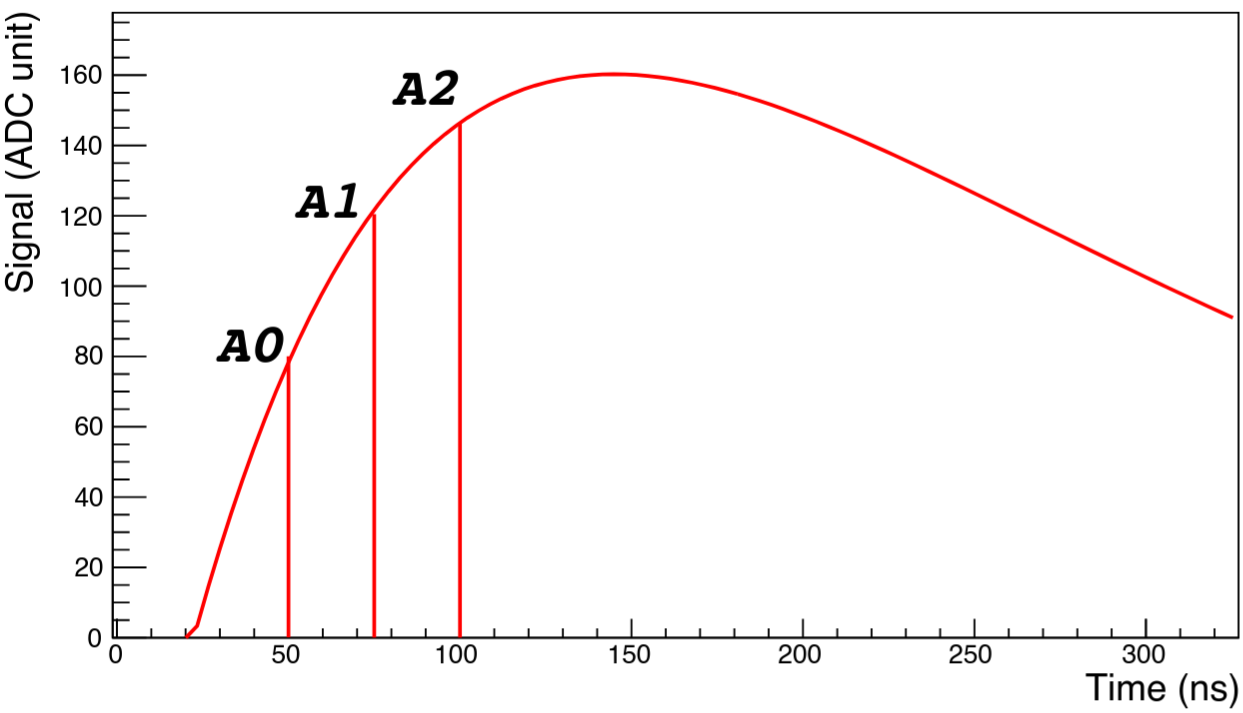
\includegraphics[width=0.45\linewidth]{images//illustrative/mm-amps.png}
    \caption{Сэмплирование переднего фронта сигнала с одного канала
    микроструктурного детектора~\cite{na64-BANERJEE201872}}
    \label{fig:apv-pulse-sampling}
\end{figure}

В рабочем режиме детектора средняя точка отвечает критерию постоянной
доле~(англ. \emph{constant fraction}~\cite{grupenDetectors2008}) и её
относительное временное смещение не зависит от
амплитуды. Поскольку у элементов входных каскадов считывающей электроники присутствует
разброс параметров, вывод детектора в рабочий режим требует
подстройки фазы синхронизирующего импульса~\acrshort{sadc}.

Для этого строится гистограмма отношений
амплитуд $r_{02}=A_0/A_2$ и $r_{12}=A_1/A_2$,
пример которой приведён на рисунке~\ref{fig:banana-histogram}. Калибровка 
заключается в выборе дискриминирующего условия на основе такого
распределения, выражающаяся в параметризованном неравенстве (обычно,
включающае полигональную фигуру, полиномы, сплайны или кривые Безье).
Таким образом исключаются паразитные
амплитуды.

\begin{figure}
    \centering
    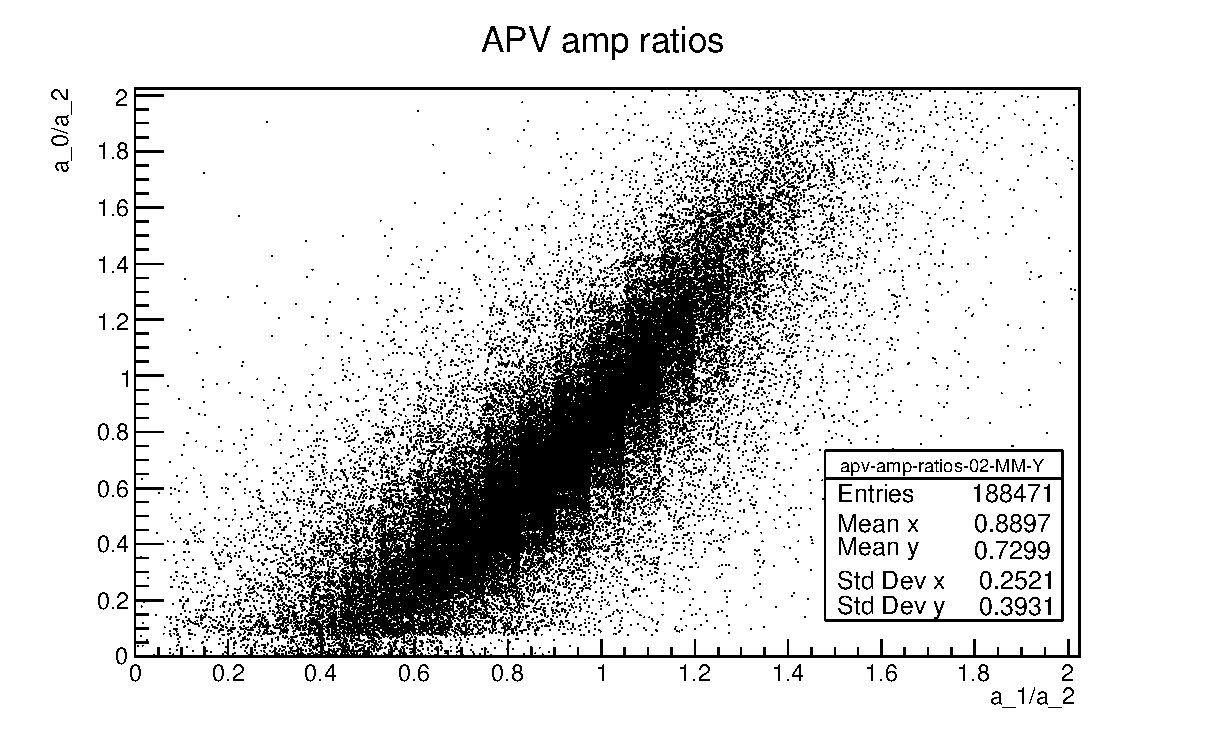
\includegraphics[width=0.45\linewidth]{images/illustrative/banana-example.eps}
    \caption{Пример распределения отношения амплитуд $r_{02}$ и $r_{12}$ переднего
    фронта сигнала микроструктурного детектора}
    \label{fig:banana-histogram}
\end{figure}

\subsection{Измерения от тонкостенных зарядовых трубок}

%Станции тонкостенных газоразрядных трубок предоставляют информацию
%о времени развития электронной лавины $t'$ в рабочем объёме конкретной
%трубки относительно времени срабатывания триггера. В $t'$ включено
%время пролёта частицы до трубки $\delta t$, которое для большинства
%релятивистских частиц (мюонов и электронов) принимается постоянным.
%Так, например, времяпролётная разница на дистанции в десять метров
%для электронов в $1~\text{ГэВ}$ и $100~\text{ГэВ}$ составляет
%менее $1~\text{пс}$, для мюонов -- менее $200~\text{пс}$, в то время
%как характерное время дрейфа лавины в трубке обычно составляет десятки
%наносекунд -- $20~\text{нс}$ для трубок диаметром $2~\text{мм}$
%и $50~\text{нс}$ для трубок $6~\text{мм}$. При принципиально-достижимом
%координатном разрешении в детекторах такого типа в $200~\text{мкм}$
%эта разница во временах для лептонов высоких энергий несущественна.
Станции тонкостенных газоразрядных трубок регистрируют время развития
электронной лавины $t'$ в рабочем объёме каждой трубки относительно
сигнала триггера. В это время включено также запаздывание
частицы $\delta t$, которое для большинства релятивистских частиц
практически постоянно. Так, например, различие
во времени пролёта на расстоянии десяти метров между электронами с
энергией $1~\text{ГэВ}$ и $100~\text{ГэВ}$ составляет менее $1~\text{пс}$,
а для мюонов~-- менее $200~\text{пс}$, тогда как характерное время
дрейфа лавины в трубке находится на уровне десятков наносекунд:
около $20~\text{нс}$ для трубок диаметром $2~\text{мм}$ и порядка
$50~\text{нс}$ для трубок диаметром $6~\text{мм}$. При достижимом
координатном разрешении таких детекторов на уровне менее $200~\text{мкм}$,
указанные различия во времени пролёта для лептонов высоких энергий
не имеют существенного значения.

%По этой причине $t'$ определяется главным образом временем $T$ дрейфа
%электронной лавины в разрядном промежутке трубки от ближайшей точки
%ионизации до катодной проволоки с расстоянием $R$, которое в свою очередь
%в наибольшей степени зависит от давления и плотности газовой смеси.
Таким образом, величина $t'$ определяется главным образом временем $T$
дрейфа электронов в разрядном промежутке трубки от ближайшей точки
ионизации до катодной проволоки.

%Таким образом зависимость $R(T)$, хотя и имеет нелинейный характер,
%хорошо поддаётся аппроксимации различными аналитическими моделями.
%Параметры такой модели и составляют необходимую калибровочную
%информацию применяемую при определении радиуса
%изохроной цилиндрической поверхности задаваемой временем срабатывания~$T$.
Функция $R(T)$ имеет нелинейный характер, однако хорошо аппроксимируется
различными аналитическими моделями. Параметры такой аппроксимации и
составляют необходимую калибровочную информацию, используемую при
определении радиуса изохронной цилиндрической поверхности, соответствующей
данному времени срабатывания~$T$.

На рисунке~\ref{fig:straws-rt} изображена гистограмма полученная для
трубки диаметром $6~\text{мм}$, находящейся
позади адронного калориметра с наложенными поверх гистограмм аппроксимациями
зависимости $R(T)$.
%\begin{figure}[ht]
%    \centering
%    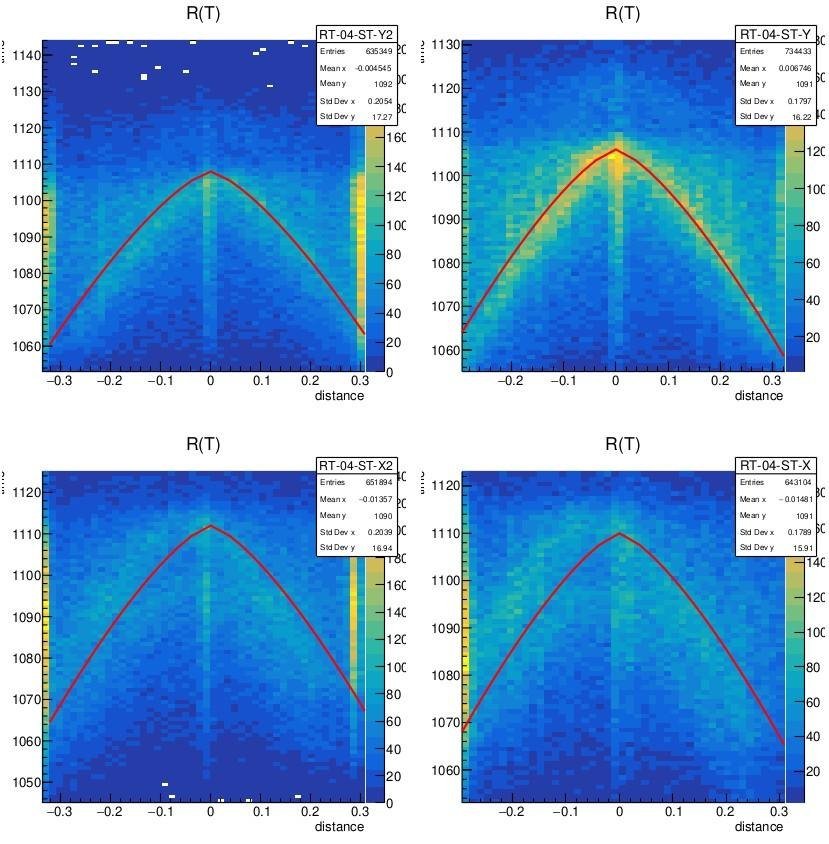
\includegraphics[width=0.95\linewidth]{images/illustrative/ST-RT.jpg}
%    \caption{Распределение $R(T)$ для нескольких трубок станции ST
%    диаметром $6~\text{мм}$ (ось времени инверирована)}
%    \label{fig:straws-rt}
%\end{figure}
\begin{figure}
    \centering
    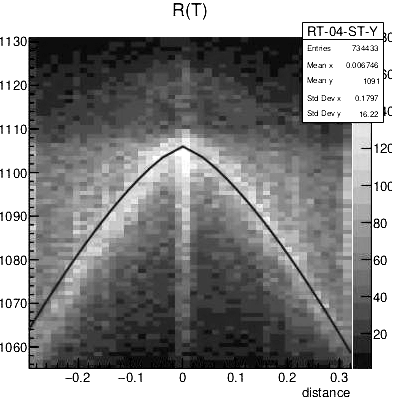
\includegraphics[width=0.33\linewidth]{images//illustrative/ST-RT-single-mono.png}
    \caption{Распределение $R(T)$ для нескольких трубок станции ST
    диаметром $6~\text{мм}$
    %, $R$ в мм, время в относительных единицах, ось времени инверирована
    }
    \label{fig:straws-rt}
\end{figure}
Большое количество срабатываний отстоящих от основной линии обусловлено
высоким фоном от вторичных частиц.

%Хотя определение радиуса изохронной поверхности таким образом представляет
%собой простую задачу (реализуемую при помощи единственного обработчика,
%применяющего калибровочные данные), последующее использование этой
%информации в
%алгоритмах трекинга требует привлечения нетривиальных
%алгоритмов либо на этапе предварительного поиска треков, либо
%в процессе подгонки параметров модели трека. В простейшем случае, проводят
%плоскость через оси трубок в одной координатной проекции, и отмечают
%линии пересечения изохронной поверхности с этой плоскостью. Получившиеся
%линии таким образом являются геометрическим местом возможного пересечения
%траектории частицы с плоскостью детектора с фиксированным разрешением.
%Поскольку для одной трубки таких линий образуется две, одной трубки
%недостаточно для определения координат частиц в одной проекции.
Хотя определение радиуса изохронной поверхности в таком подходе
представляет собой относительно простую задачу (реализуемую с помощью
единственного обработчика, использующего калибровочные данные),
дальнейшее применение этой информации в алгоритмах трекинга требует
привлечения более сложных методов -- как на этапе предварительного
поиска треков, так и при подгонке параметров модели трека. 

В простейшем случае через оси трубок в одной координатной проекции
проводится плоскость, и фиксируются линии пересечения изохронной
поверхности с этой плоскостью. Эти линии образуют геометрическое
место возможных точек пересечения траектории частицы с плоскостью
детектора при данном временном разрешении. Поскольку для одной трубки
возникают две такие линии, её информации недостаточно для определения
координаты частицы в одной проекции. Тем не менее, рассматривая показания
трековых детекторов в совокупности зачастую удаётся разрешить
возникающие неоднозначности. На рисунке~\ref{fig:evdisplay-new}
показана проекция пространственных примитивов изображающих
чувствительные объёмы детекторов MicroMega и станции трубок
совместно с допустимыми пределами разрешений (изображены
шириной $5\sigma$).

\begin{figure}[ht]
    \centerfloat{
        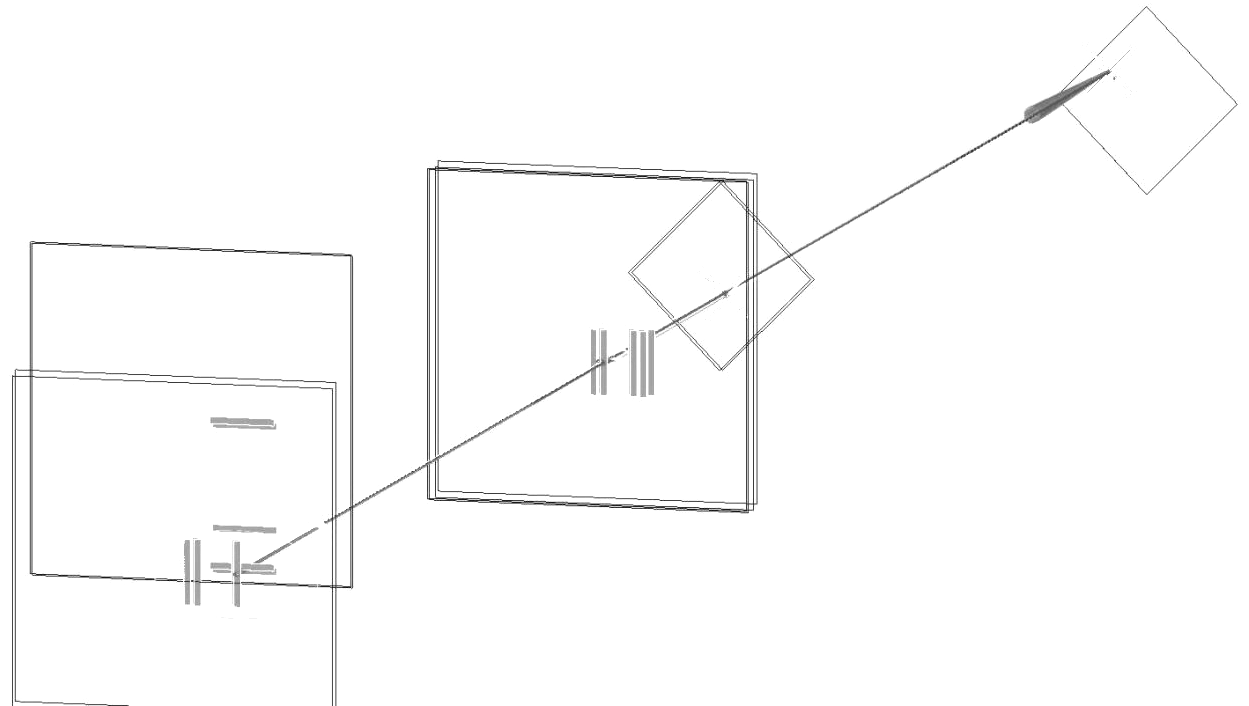
\includegraphics[width=0.5\linewidth]{images//illustrative/ST-evdisp-mono.png}
    }
    \caption{Реконструкция треков по показаниям MicroMega (повёрнуты на $45^{\circ}$)
    со станциями тонкостенных разрядных трубок с изображением
    координатных разрешений и гипотезы трека с ковариационными конусами}
    \label{fig:evdisplay-new}
\end{figure}

%\begin{figure}
%    \centering
%    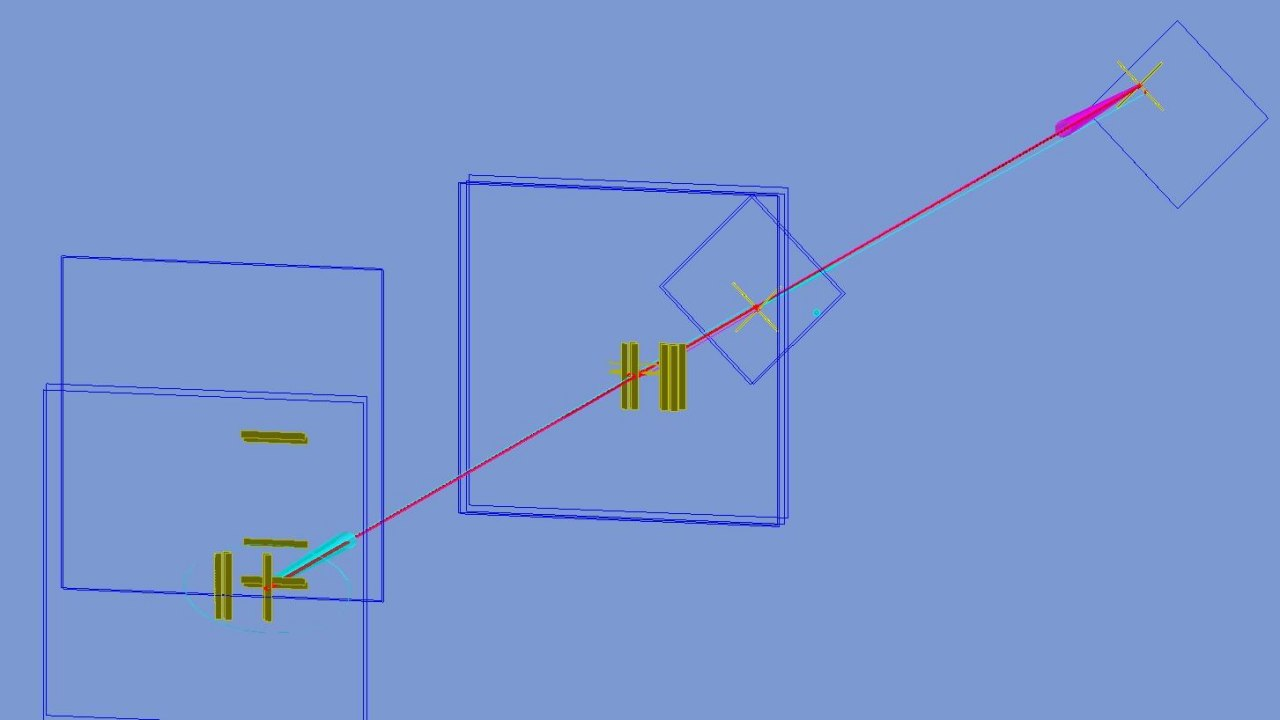
\includegraphics[width=0.5\linewidth]{images/illustrative/ST-evdisp.jpg}
%    \caption{Реконструкция треков в SPA}
%    \label{fig:evdisplay-new}
%\end{figure}

Возможны и более сложные алгоритмы реконструкции, учитывающие
трёхмерную структуру изохронных поверхностей в рамках одной станции
тонкостенных трубок~\cite{straws-peshekhonov2015}.

\subsection{Алгоритмы аппроксимация треков}

Классическая задача восстановления трека по измеренным
координатам в NA64 решалась различными методами.
Наиболее актуальным является фильтр Калмана~\cite{kalman-1960},
реализованный библиотекой GenFit2~\cite{Genfit2_Rauch_2015}
в различных редакциях и с дополнениями оригинального алгоритма, из которых
наибольший практический интерес в контексте NA64
представляют
\acrshort{daf} (англ. \emph{deterministing annealing filter}~\cite{daf-track-fitting})
и \acrshort{krf}
(англ. \emph{Kalman filter with reference track}~\cite{krf-kalman-w-reference-track}).

Для подгонки параметров модели треков в условиях сложной геометрии
применяется \acrshort{krf}.
Его особенность по сравнению с оригинальным алгоритмом Калмана
состоит в том, что линеаризация функции описывающей движение
частицы выполняется не в малой окрестности координатного измерения, а
относительно заранее заданной опорной траектории,
обновляемой затем в несколько итераций. Этот приём позволяет снизить
систематические ошибки при аппроксимации трека в
неоднородном магнитном поле, с учётом эффектов множественного
рассеяния (например, при трассировке участка трека через калориметр).
Использование данного метода оправданно в сочетании с алгоритмами
поиска треков, которые задают разумное начальное приближение
для опорной траектории. % -- таких, как CATS~\cite{catsc-nim}.

\acrshort{daf} решает иную задачу: выбор согласованного подмножества
измерений в условиях неоднозначностей и шумов. В
его основу положено назначение весов отдельным координатным измерениям
с последующим итеративным обновлением. Таким образом, вначале все
измерения вносят вклад в гипотезу о треке частицы, затем, в течение
нескольких итераций, веса
асимптотически сходятся к самосогласованной гипотезе.
В пределе это приводит к отбору хитов, принадлежащих
правдоподобной гипотезе с эффективным исключением ложных
срабатываний.

\subsection{Задача предварительного поиска треков}

%Задача предварительного поиска треков (англ. \emph{pattern recognition})
%состоит в выборе таких комбинаций пространственных объектов соответствующих
%отдельным измерениям, которые с заданной
%степенью правдоподобия могут образовывать трек частицы.
Задача предварительного поиска треков % (англ. \emph{pattern recognition})
заключается в отборе таких комбинаций пространственных объектов,
соответствующих отдельным измерениям детектора, которые с заданной
степенью правдоподобия могут образовывать трек частицы.


%Среди множества существующих на сегодняшний день алгоритмов предварительного
%поиска треков~\cite{MankelTracking}, интерес представляет алгоритм
%CATS~\cite{catsc-JINR, catsc-discrete, catsc-nim, catsc-disto},
%(англ. \emph{cellular automata track search} -- в разное время авторы
%публиковали его формализацию в терминах <<эластичных>> нейронных сетей,
%и клеточных автоматов), который допускает весьма общую
%формулировку в силу независимости по отношению к конкретным
%геометрическим свойствам входных данных.
Среди многочисленных алгоритмов предварительного поиска~\cite{MankelTracking}
интерес представляет метод CATS\footnote{В различных публикациях
он излагался как в терминах <<эластичных>> нейронных сетей,
так и в формализме клеточных автоматов.}
(англ. \emph{cellular automata track search})~\cite{catsc-JINR, catsc-discrete, catsc-nim, catsc-disto}.
Алгоритм допускает весьма общую формулировку в силу независимости по
отношению к конкретным геометрическим свойствам входных данных.

Формально задача, решаемая алгоритмом, может быть представлена следующим образом.
Пусть имеется
набор объектов $h_1,h_2, ...h_n$ (англ. \emph{hit}). Требуется найти такие
последовательности $(h_i,h_j,...h_m)$, для которых любая тройка
элементов $(h_{i-1},h_{i},h_{i+1})$ удовлетворяет заданному
условию $F(h_{i-1},h_{i},h_{i+1})=1$.
Основная идея состоит в эффективной стратегии обхода
объектов~$h$, позволяющей в большинстве случаев избежать прямого перебора
всех возможных комбинаций. Для этого алгоритм опирается на
топологическую информацию о <<слоях>> связанных с каждым
объектом~$h$. Каждому объекту сопоставляется
внутреннее состояние, обновляемых за конечно число итераций согласно
определённому правилу.

Пример работы алгоритма показан на рисунке~\ref{fig:catsc-nim},
где приведены начальное и конечное состояния графа для
синтетических данных.

\begin{figure}
    \centerfloat{
        \hfill
        \subcaptionbox{Начальное состояние}{
            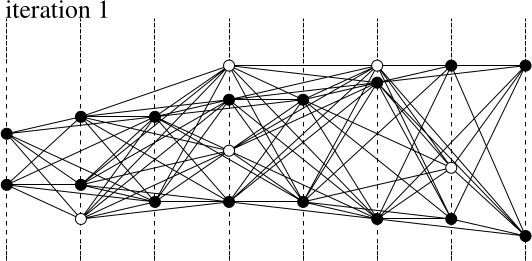
\includegraphics[width=0.45\linewidth]{images//illustrative/catsc-quote-it1.png}}
        \hfill
        \subcaptionbox{Конечное состояние}{
            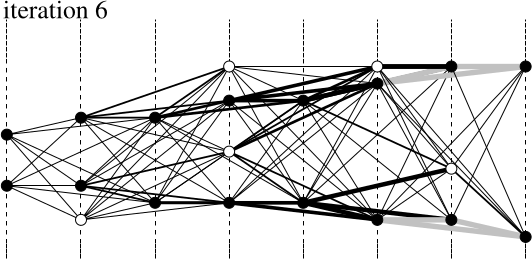
\includegraphics[width=0.45\linewidth]{images//illustrative/catsc-quote-it6.png}
        }
        \hfill
    }
    \legend{Слои отмечены пунктирными
    линиями, объекты $h$ изображены кругами, рёбра между парами
    объектов~--- сплошными линиями, а увеличенная толщина линии указывает
    на больший вес соответствующей пары.}
    \caption{Пример работы клеточного автомата CATS~\cite{catsc-nim}}
    \label{fig:catsc-nim}
\end{figure}

В простейшем случае, в качестве объектов $h$ выбираются пространственные
точки, а условием $F$ является условие на максимальный пространственный
между ними $F(h_{i-1},h_{i},h_{i+1}): \angle(h_{i-1}h_i) (h_i h_{i+1}) < \theta_{th}$.

В результате время работы алгоритма оказывается существенно ниже
прямого перебора, в худшем случае ($\theta_{th} =\pi$) имея
сложность $\mathcal{O}(Ln^3)$, где $L$ -- число слоёв,
и $n$ -- число объектов $h$. Практически, сложность регулируется
функцией-фильтром, и при трудоёмкости фильтра~$\mathcal{O}(1)$ алгоритм
имеет сложность $\mathcal{O}(Ln^2)$. Наивный перебор троек $h$
с фильтрующей функцией дающей в среднем $d$ объектов в следующем слое
имеет сложность $\mathcal{O}(n^3 d^{L-3})$. Без фильтрующей функции
максимальная сложность возрастает экспоненциально $\mathcal{O}(n^L)$,
однако главное преимущество CATS перед наивной реализацией состоит
в устранении экспоненциального роста памяти, необходимой для хранения
гипотез. Алгоритм сводит задачу к итеративному однонаправленному обходу
двунаправленного графа без рекурсии.

В оригинальных работах~\cite{catsc-JINR, catsc-discrete, catsc-nim, catsc-disto}
$h_i$ рассматриваются как пространственные точки $h_i:=\vec{r}_i$, или кортежи из
координат и времени $h_i:=(\vec{r}_i,t_i)$, в то время как алгоритм сам по себе
не подразумевает какого-то конкретного набора свойств, а требует
только того, чтобы определена функция $F:h_{1,2,3} \rightarrow \{0,1\}$.

Дополнением оригинального алгоритма является определение весовых
коэффициентов возвращаемых функцией-фильтром, то есть в более общем
случае $F: F(h_{1,2,3}) =w_j, ~w_j \in \mathbb{R_1}$. Кроме того, после
конструирования графа связности, стратегия извлечения гипотез (обхода точек)
может допускать различные формы, что в оригинальных работах не
рассматривается. В частности, в случае когда одна и более гипотез $T_p, T_q$
претендуют на один и тот же сегмент $T_p \cap T_q = (h_i, h_j)$ выбор в пользу
той или иной гипотезы целесообразно бывает разрешать руководствуясь различными
критериями. Стратегии обхода результирующего графа реализованы в виде
программных модулей.

\subsection{Результаты}

Детекторы и система сбора данных NA64 принципиально способны
регистрировать события с высокой множественностью треков
(до нескольких сотен). Однако, без применения алгоритмов
предварительного выбора гипотез, восстановление
трека алгоритмами типа \acrshort{daf} позволяет получить усреднённое представление
о треках частиц, с потерей существенной части физической информации.
На рисунке~\ref{fig:muon-momenta-test-histogram}
приведён спектр треков мюонов, восстановленных с помощью алгоритма
\acrshort{daf} при высокой интенсивности пучка
(порядка $10^6$ мюонов в секунду).
\begin{figure}[h]
    \centerfloat{
        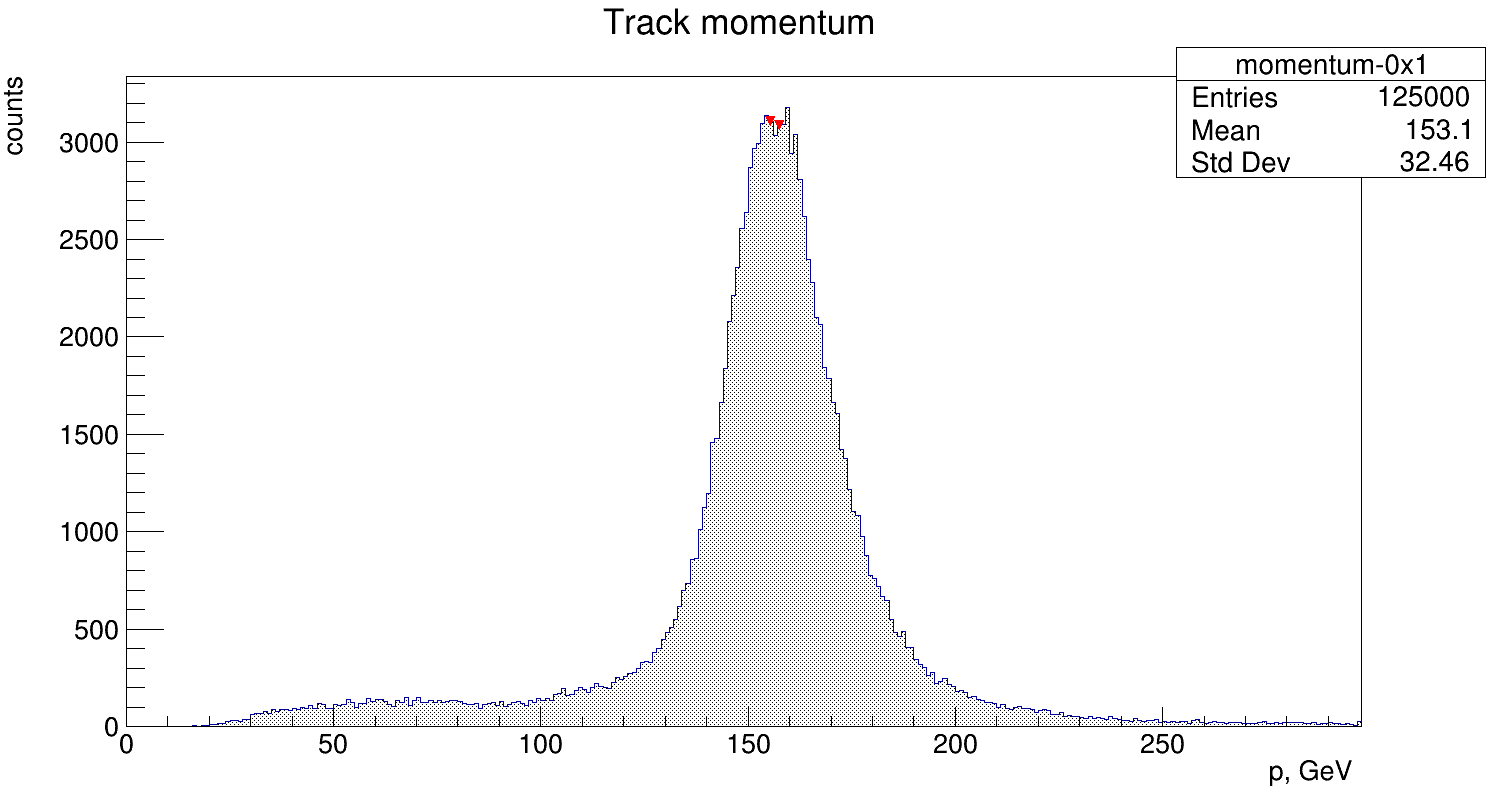
\includegraphics[width=0.65\linewidth]{images//illustrative/momentum-reco-example.png}
    }
    \caption{Спектр мюонов реконструированных алгоритмом \acrshort{daf} без
    предварительного выбора гипотез}
    \label{fig:muon-momenta-test-histogram}
\end{figure}
Пьедестал спектра в основном соответствует случайной сходимости
алгоритма на правдоподобных комбинациях координатных измерений,
без учёта конкурирующих гипотез и дополнительных предположений о
правдоподобии.

Использование алгоритма CATS для выделения треков частиц
позволяет эффективно исключить некорректные гипотезы, согласно
некоторому геометрическому критерию. При заданной принадлежности
объектов $h_p,h_q,h_r$ идущим по порядку
слоям $h_p\in l_{i-1}, h_i \in l_i, h_p\in l_{i+1}$ критерий $F(h_{p}, h_q, h_{r}) \in [0,1]$ может включать произвольное условие.

\subsection{Результаты CATS(C) на модели данных Belle~II}

В качестве примера, помимо простейшего теста на принадлежность угла
$\angle(h_p,h_q),(h_q,h_r)$ заданному диапазону, можно рассмотреть
постановку задачи в соленаодиальном поле баррельной части коллайдерного
детектора, в рамках которой функция-фильтр $F$ должна проверять
гипотезу о спиральной траектории заряженных частиц в смысле некоторых
регулярных геометрических свойств. Например, в цилиндрической системе
координат $(\rho, \phi, z)$, выбирая попарные комбинации из триплета $h_{p}, h_q, h_{r}$,
можно проверять шаг $\lambda_{ij} = \Delta z_{ij}/\Delta \phi_{ij}$
на приблизительное равенство относительно некоторого порога $\epsilon$:
\begin{align}
    F(h_{p}, h_q, h_{r}) = |\lambda_{12} / \lambda_{23} - 1| <\epsilon ~
    \wedge |\lambda_{12} / \lambda_{13} - 1| <\epsilon.
\end{align}

Результаты моделирования в геометрии Belle~II~\cite{belle-ii} изображены на
рисунке~\ref{fig:belle-ii-mc-event}.
\begin{figure}[ht]
    \centerfloat{
        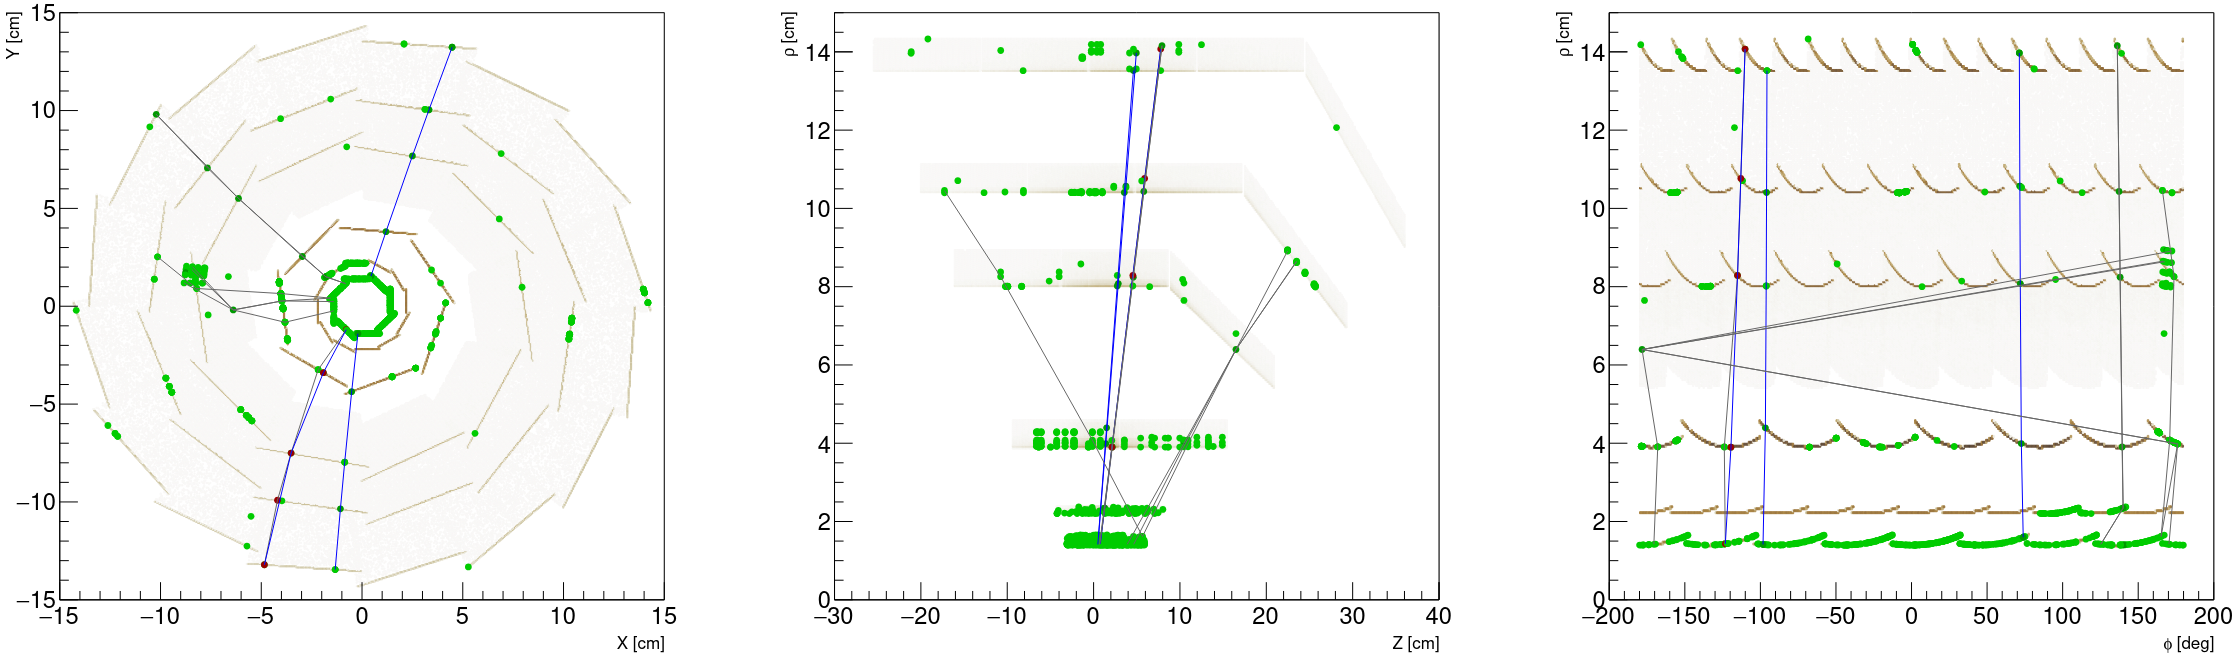
\includegraphics[width=1\linewidth]{images//illustrative/belle-ii-mc-event.png}
    }
    \legend{Поверх схематичного изображения детекторов
внутреннего и внешнего трекера зелёным нанесены точки, соответствующие
измерениям детекторов $h$, синими линиями соединены найденные треки,
соответствующие истинным траекториям, реконструированным алгоритмом;
серым -- комбинации отвечающие ложным гипотезам.}
    \caption{Результат применения реализации CATS(C) на данных \acrshort{mc}-моделирования
    одного сособытия геометрии детектора Belle II~\cite{belle-ii} 
    (автор -- С.~Герасимов}
    \label{fig:belle-ii-mc-event}
\end{figure}

На рисунке \ref{fig:belle-ii-catsc} приведены результаты моделирования
для Belle~II, откуда для заданного уровня статистической значимости можно получить
ограничения на значения различных порогов функции-фильтра.
Заметно, что значения, соответствующие истинным трекам размываются благодаря множественному рассеянию.

\begin{figure}
    \centerfloat{
        \subcaptionbox{Отношение спирального шага $\lambda_{12}/\lambda_{23}$}{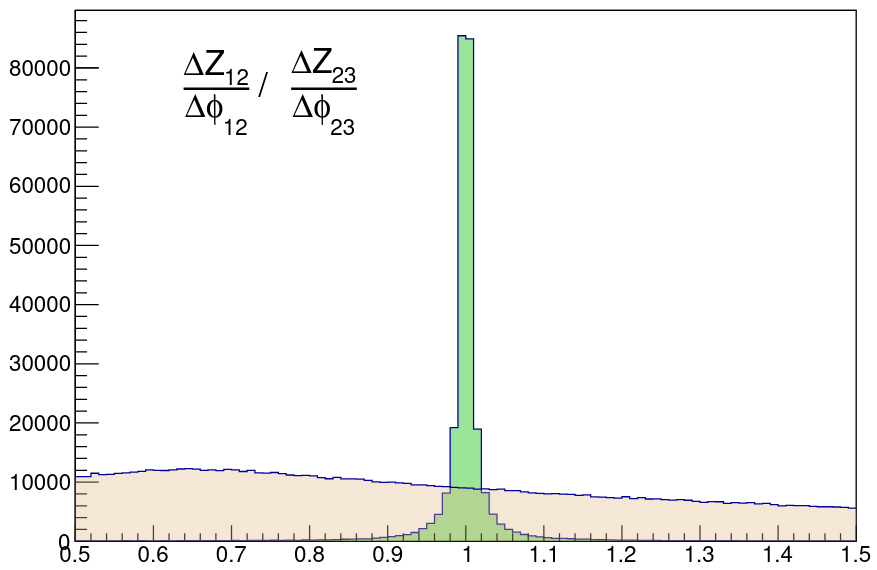
\includegraphics[width=0.32\linewidth]{images//illustrative/pitch-ratios.png}}
        \subcaptionbox{Продольный угол $\alpha_{12-23}$}{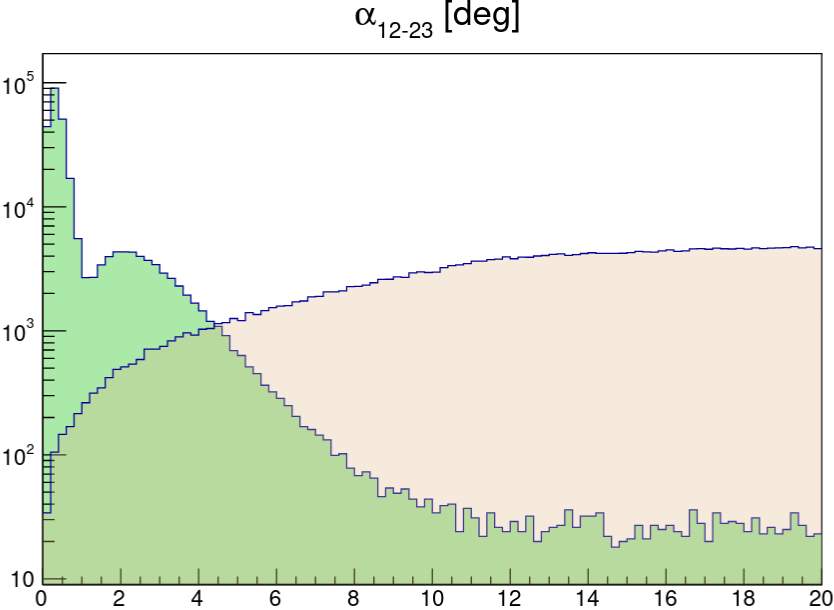
\includegraphics[width=0.3\linewidth]{images//illustrative/belle-ii-catsc-opening-angle.png}}
        \subcaptionbox{Разница спиральных шагов
    $\lambda_{12} - \lambda_{23}$}{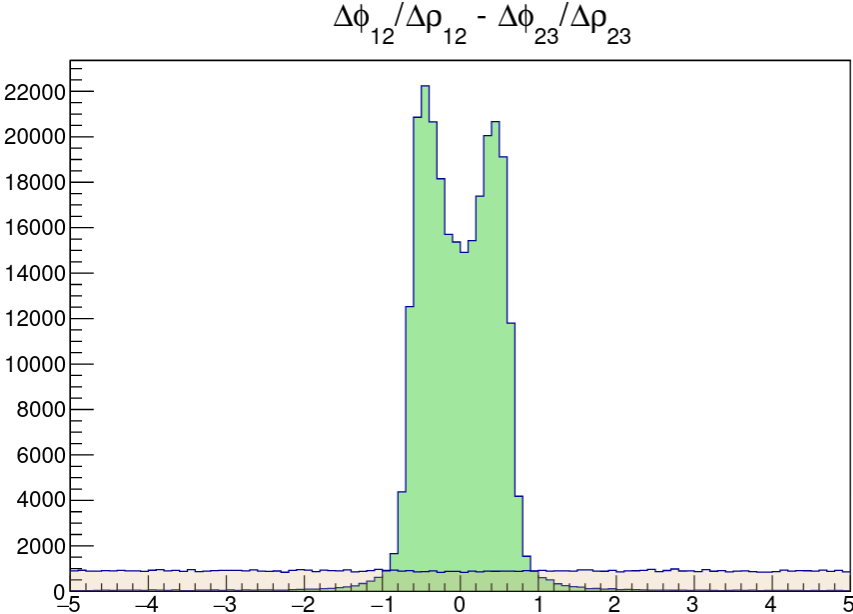
\includegraphics[width=0.32\linewidth]{images//illustrative/belle-ii-catsc-pitch-delta.png}}
    }
    \legend{Зелёным цветом выделены значения,
    соответствующие истинным трекам, комбинаторный фон обозначен жёлтым}
    \caption{Распределения спиральных геометрических характеристик триплетов,
    по результатам \acrshort{mc}-моделирования
    Belle~II для оценки мощности критерия~(С.~Герасимов)}
    \label{fig:belle-ii-catsc}
\end{figure}

\subsection{Результаты CATS(C) данных $\text{NA64}\mu$}

Результаты применения алгоритма для реконструкции треков $\text{NA64}\mu$ приведены на
рисунке~\ref{fig:cats-impact-na64}.
\begin{figure}[ht]
    \centerfloat{
        \hfill
        \subcaptionbox{}{
            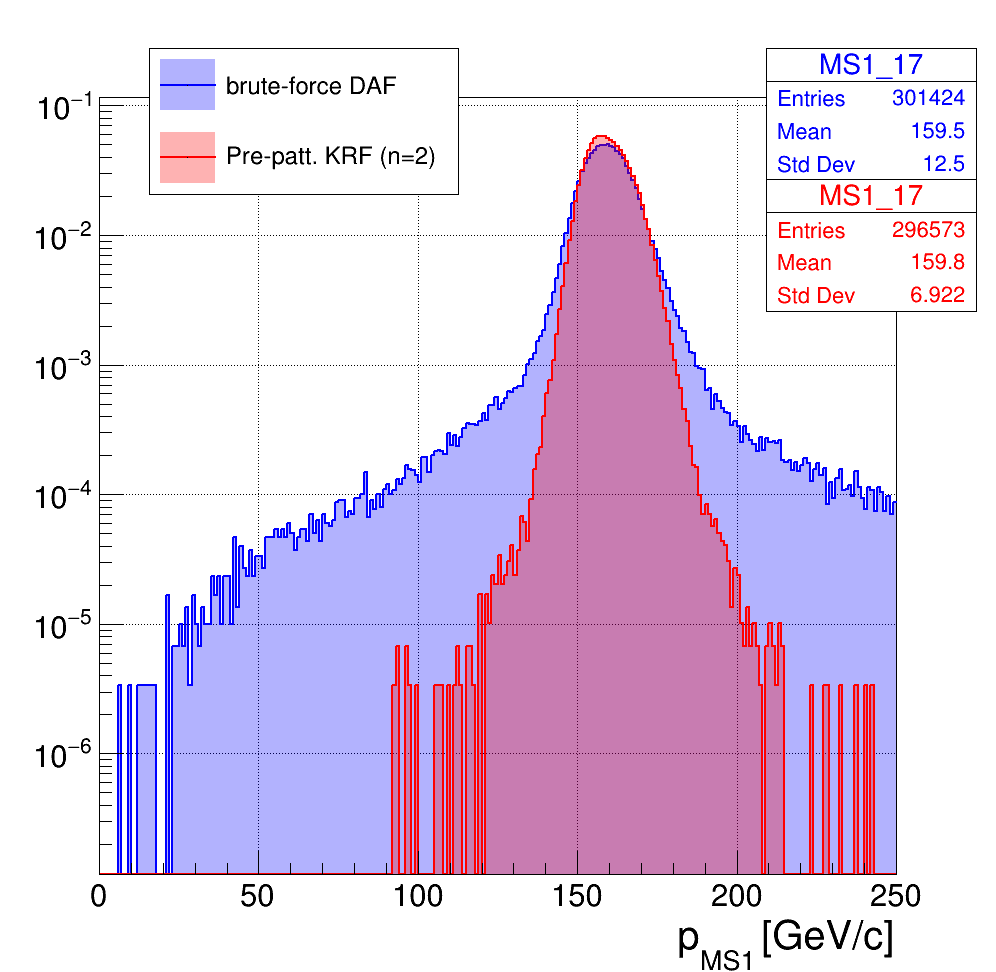
\includegraphics[width=0.49\linewidth]{images//illustrative/catsc-impact.png}
        }
        \hfill
        \subcaptionbox{}{
                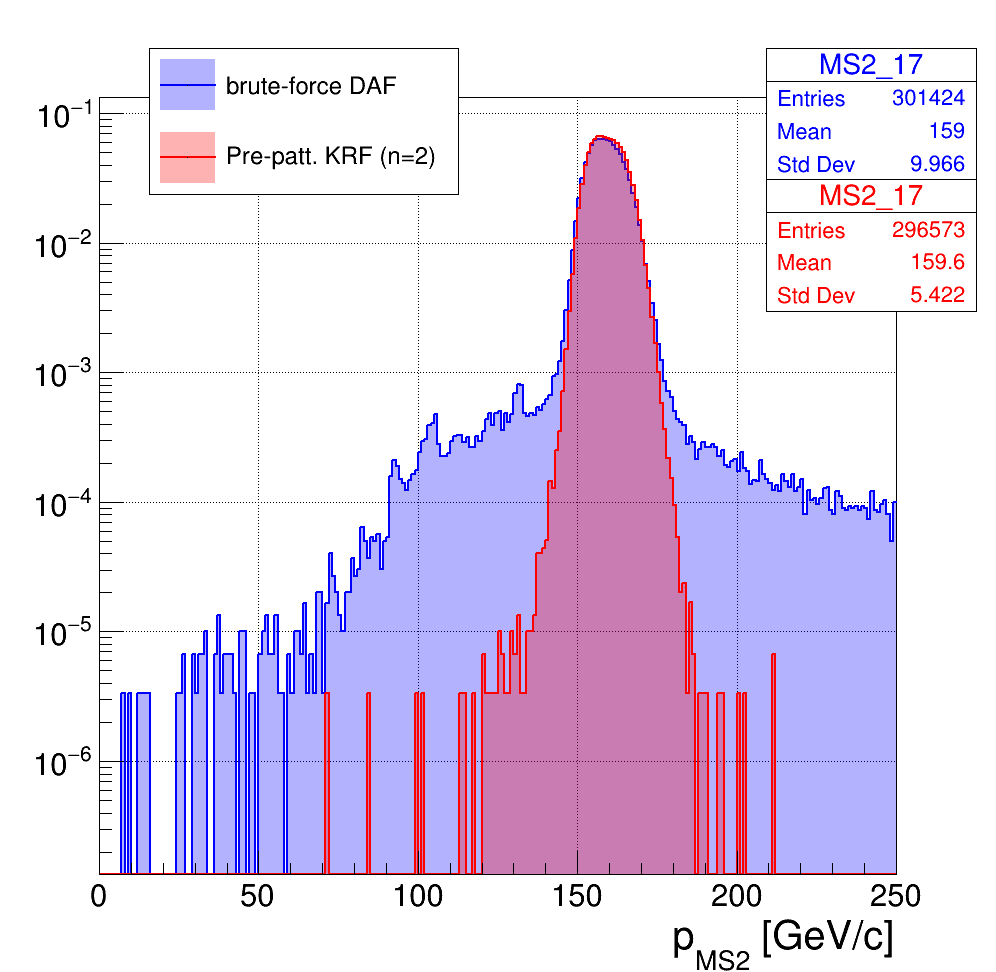
\includegraphics[width=0.49\linewidth]{images//illustrative/catsc-impact-2.png}
        }
        \hfill
    }
    \caption{Распределение импульсов частиц NA64mu реконструированных при
    помощи DAF без применения CATS(C) и при помощи KRF после CATS(C)
    до (MS1) и после (MS2) основного магнита спектрометра NA64mu~(автор -- M.~Tuzi)}
    \label{fig:cats-impact-na64}
\end{figure}
В постановке NA64mu применение алгоритма для предварительного отбора гипотез треков
особенно важно, поскольку участок установки MS2 находится после электромагнитного
калориметра, и трекер должен разрешать траектории при повышенной
загрузке (в среднем $\simeq 10$ треков на событие против $\simeq 1.4$ в MS1)
от вторичных частиц после ECAL.

При консервативной оценке пороги для углов или спирального шага
регулируют в основном количество избыточных гипотез найденных алгоритмом, которые
затем отсеивают при подгонке треков и проверки более строгих гипотез. Избыточные
гипотезы можно ограничить на основе оценок порогов полученных с
применением \acrshort{mc}-моделирования, или при помощи консервативных
геометрических оценок.

В некоторых случая можно прибегнуть к упрощённому рассмотрению.
Рисунок~\ref{fig:na64-cutoff-angle} иллюстрирует распределение углов
для допустимых триплетов $h$ в пределах $3\sigma$, где $\sigma$ -- пространственное
разрешение одной станции. Видна существенная (вплоть до кратности $\times5$) разница
углового порога.
\begin{figure}[ht]
    \centering
    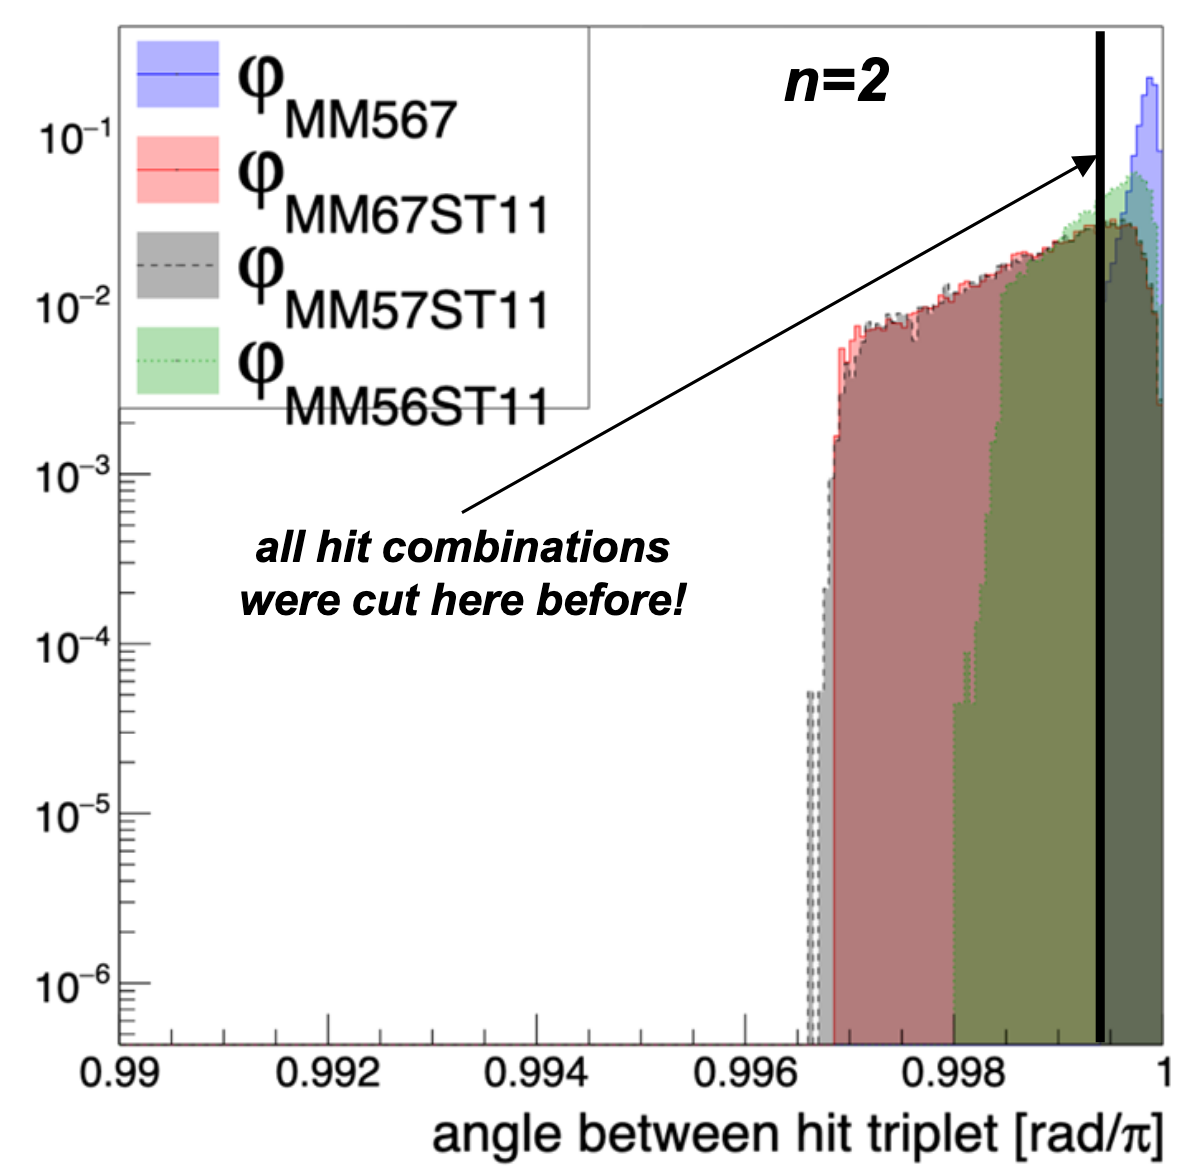
\includegraphics[width=0.5\linewidth]{images//illustrative/na64-cutoff-effic.png}
    \caption{Распределение углов для всех возможных комбинаций при учёте разрешения
    отдельных станций трекера MS2 NA64mu~(M.Tuzi)}
    \label{fig:na64-cutoff-angle}
\end{figure}

\subsection{Количественные оценки качества восстановления треков}

%Задача восстановления треков частиц по данным зачастую формулируется
%как минимизация функционала, в котором в качестве метрического значения
%выбирается величина, пропорциональная отклонению ожидаемых значений
%от фактически измеренных. Для многих детекторов статистика таких
%отклонений (ошибок), отнесённых к абсолютному разрешению детектора,
%подчиняется распределению~$\chi^2$.

%\begin{figure}[ht]
%    \centering
%    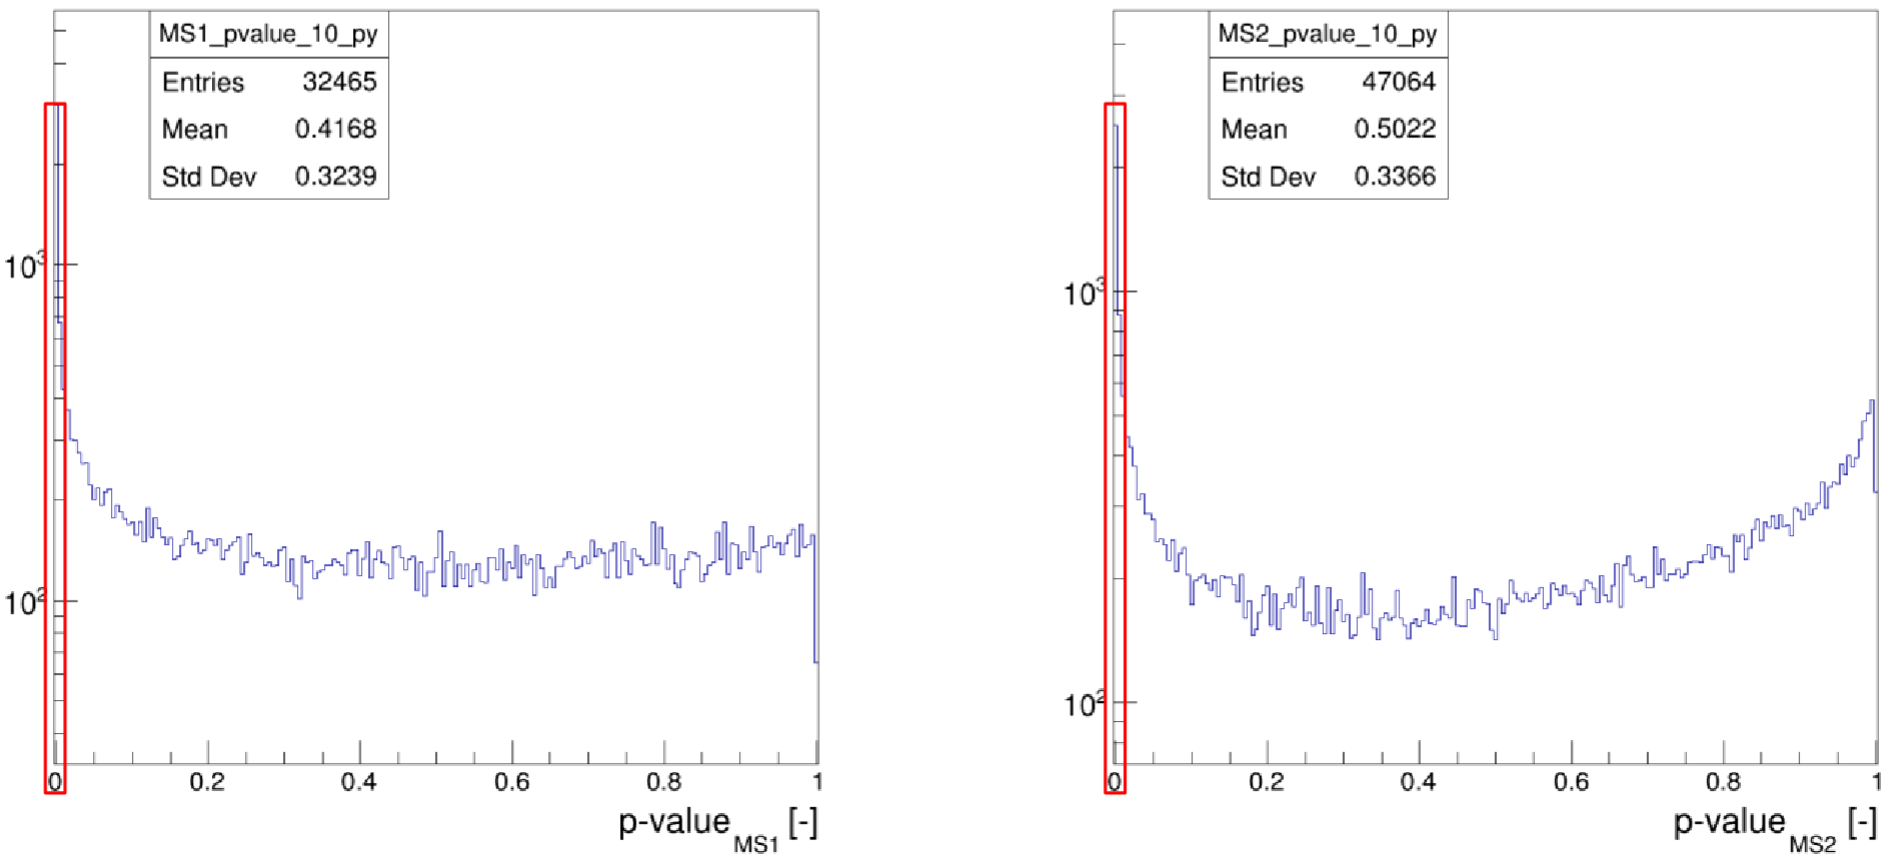
\includegraphics[width=1\linewidth]{images//illustrative/na64-p-value-before-truly.png}
%    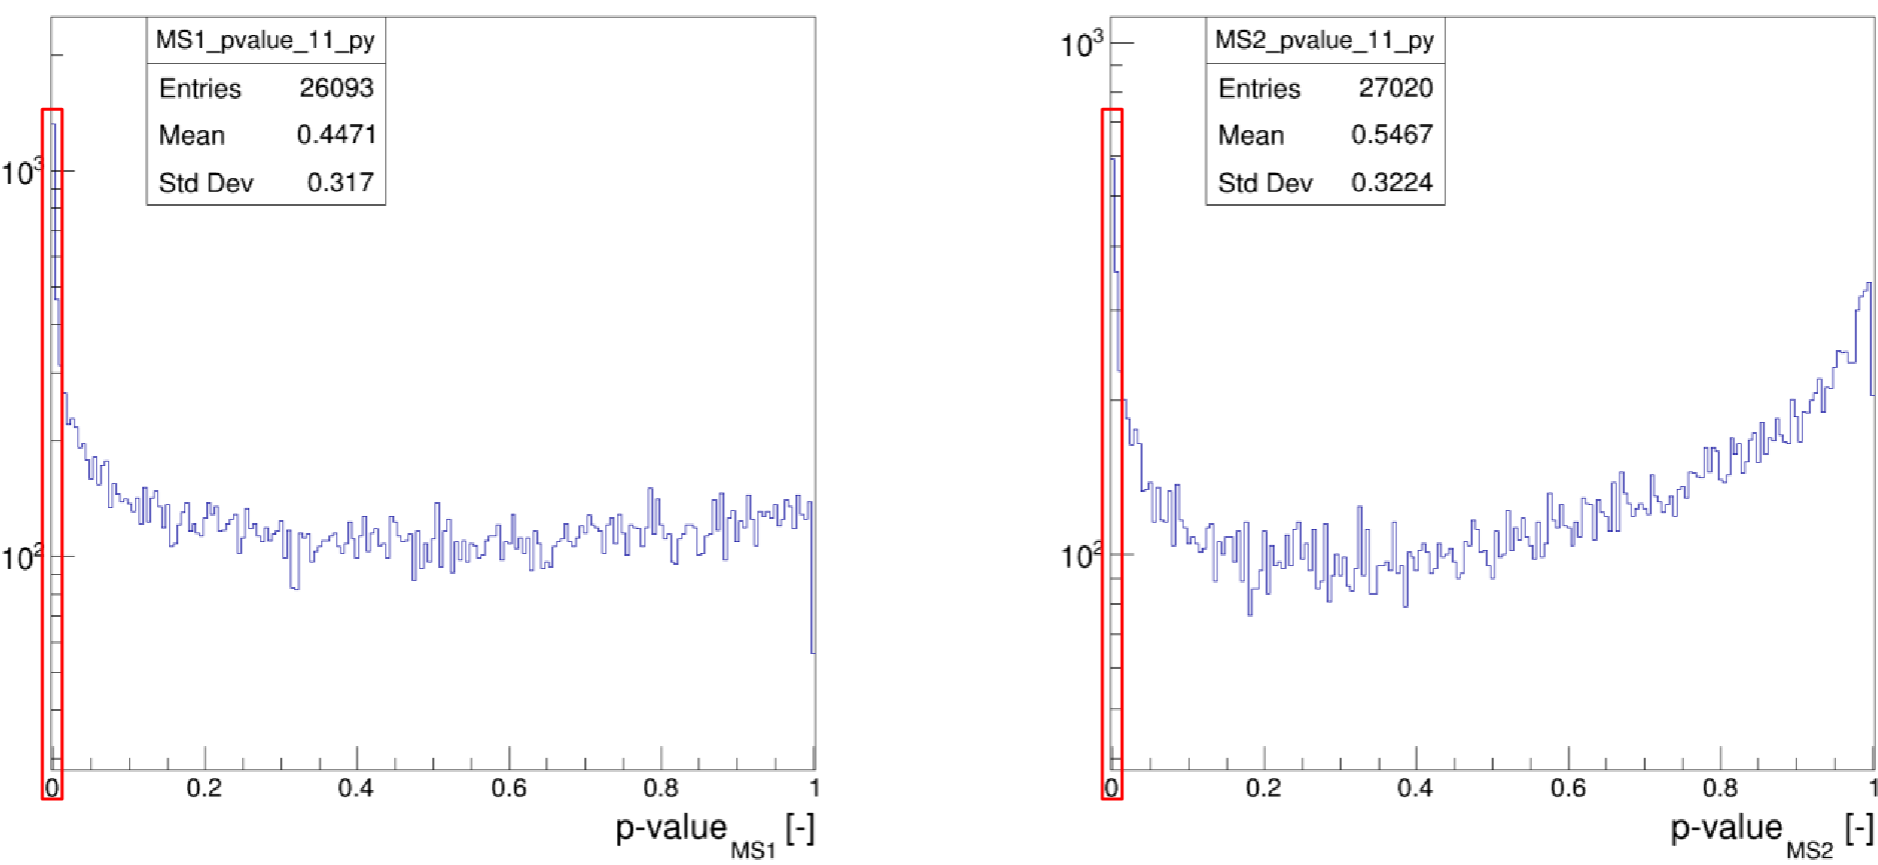
\includegraphics[width=1\linewidth]{images//illustrative/na64-pvalue-before.png}
%    \caption{Распределение $p_{\chi^2}$ реконструированных треков для плечей мюонного спектрометра NA64 до и после учёта wire layout~(M.Tuzi)}
%    \label{fig:na64-muon-p-value-distribution}
%\end{figure}

Важным фактором, влияющим на качество восстановления треков, является
соответствие предполагаемых положений детекторов фактическим. Для
оценки этого соответствия в случае индивидуальных детекторов строят
распределения координатных невязок (англ. \emph{residuals}) в
системе локальных координат, связанной с детектором.
Для стриповых и проволочных детекторов (измеряющих координату в
одном направлении) используют одно направление ($u$), выбираемое
соответствующим измеряемой координате, второе обычно
перпендикулярно ему.

При ориентации плоскости перпендикулярно пучку распределение невязок
характеризует ошибку в определении позиции центра
координатной плоскости детектора в поперечных координатах (вдоль $u$).
Для получения более детализированной картины строят
распределение $\delta u/dv$, естественно характеризующее ошибку в определении
угла поворота, перпендикулярного направлению пучка. Распределение
$\delta u/du$ характеризует ошибку в определении продольной координаты.

На рисунке~\ref{fig:residuals-example} показан пример комплексного
графика, характеризующего распределение невязок $\delta u$ против $v$.
\begin{figure}[ht]
    \centering
    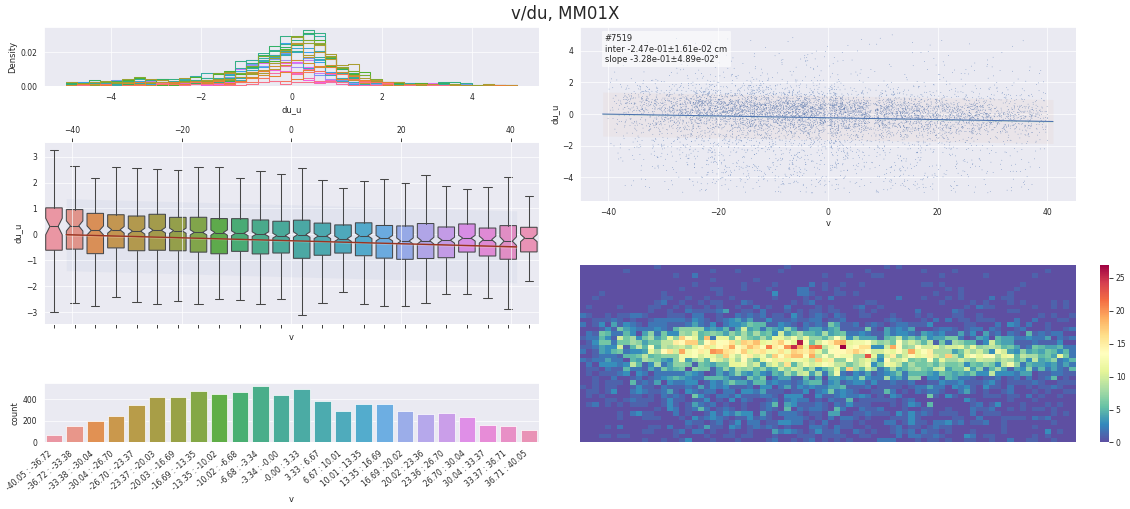
\includegraphics[width=0.95\linewidth]{images/illustrative/alignment-example.png}
    \caption{Комплексный график иллюстрирующий распределение координатных
    невязок $\delta u /v$ для плоскости X первой станци MicroMega}
    \label{fig:residuals-example}
\end{figure}

Такое изображение координатных невязок можно использовать, в частности,
в процедуре выравнивания детекторов по \emph{несмещённым} невязкам, когда
среди всего набора выбирается пара опорных детекторов $P_1,~P_2$, по отношению
к которым производят итеративное выравнивание. Включая в процедуру
реконструкции по одному детектору последовательно, для каждого уточняют
значения позиций и углов на основе распределений подобных изображённым
на рисунке~\ref{fig:residuals-example} при условии, что рассматриваемый
в данный момент детектор не используется для реконструкции треков (однако,
программный комплекс рассчитывает для него координатные невязки).

Подобные изображения координатных невязок используются, в частности,
в процедуре выравнивания детекторов по \emph{несмещённым} невязкам.
В такой процедуре из всего набора выбирается пара опорных детекторов,
относительно которых проводится итеративное выравнивание.
Для каждого отдельного детектора уточняют положения и углы на основе распределений,
подобных показанным на рисунке~\ref{fig:residuals-example}, при условии,
что данный детектор не используется для реконструкции треков (однако
программный комплекс вычисляет для него координатные невязки). После
выравнивания очередного детектора, он добавляется к опорным, и переходят
к следующему.

Процедура выравнивания по \emph{смещённым} невязкам, напротив,
предполагает включение всех корректируемых детекторов в реконструкцию трека.
В этом случае линеаризованные невязки образуют блочную матрицу,
которую можно использовать для решения \acrshort{sle}.

В программном окружении реализованы инструменты
для обеих процедур физического выравнивания и оценивания качества
реконструкции треков частиц. Инструменты для выравнивания по
несмещённым невязкам (графики и регрессионные модели) реализованы
в парадигме отдельных обработчиков ковейерного паттерна, выравнивание
по смещённым невязкам реализовано в виде специализированных
обработчиков и специализированной утилиты для помещения их вывода
на вход процедуры обращения блочных матрицы
Millipede~II~\cite{millipede-blobel2009}.

На рисунке~\ref{fig:na64-muon-p-value-distribution} показаны распределения $p$-значений
(интегральных вероятностей $\chi^2$) в плече MS1. Вид этого распределения
используется для косвенной оценки качества работы трекера. В случае полного
соответствия фактических разрешений детекторов установки номинальным,
распределение должно быть плоским. Увеличение популяции справа
($p_{\chi^2} \rightarrow 1{,}0$) означает, что разрешение одной или нескольких
станций оценивается пессимистически (фактическое меньше ожидаемого).
\begin{figure}[ht]
    \centering
    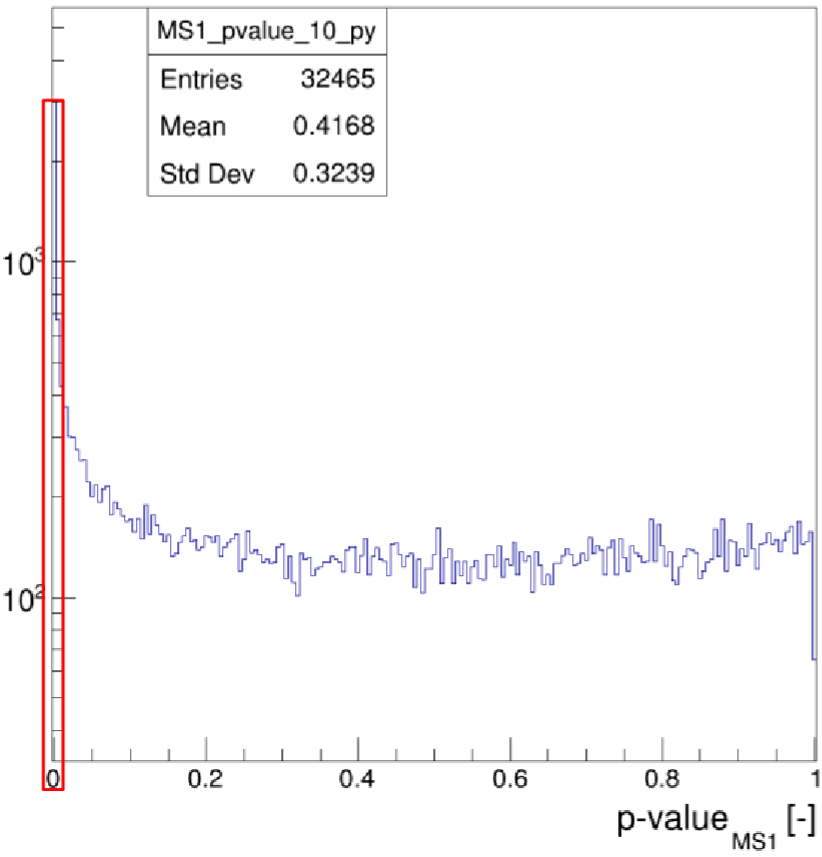
\includegraphics[width=0.5\linewidth]{images/na64-ms1-p-value-before.png}
%    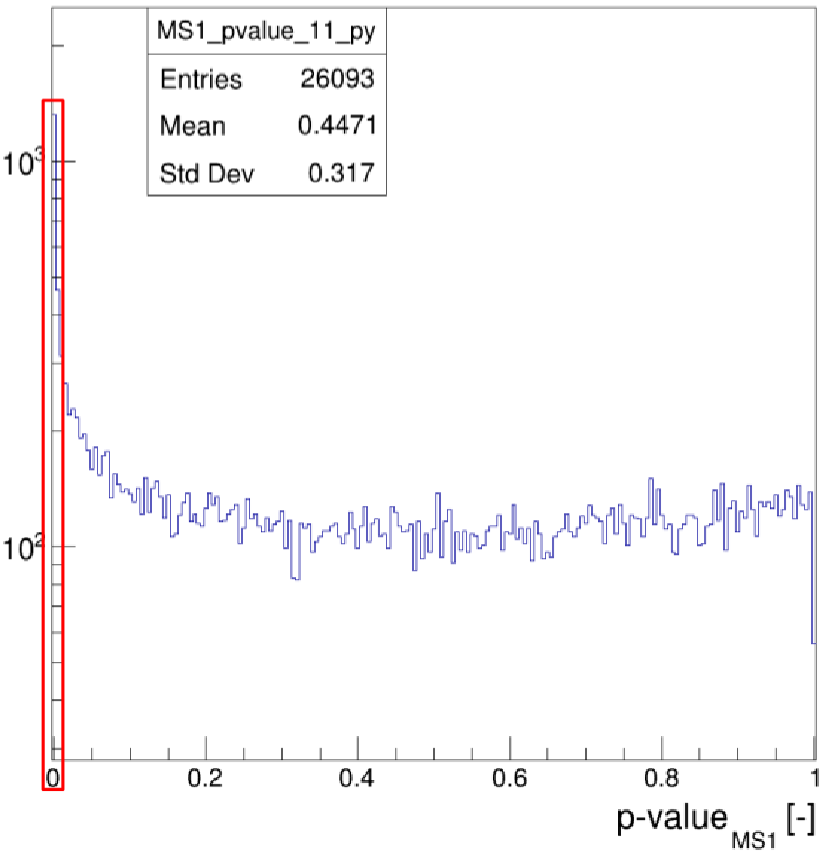
\includegraphics[width=0.5\linewidth]{na64-muon-p-value-ms1-dist-after.png}
    \caption{Распределение $p_{\chi^2}$ реконструированных треков в плече MS1 мюонного спектрометра NA64 после выравнивания~(M.Tuzi)}
    \label{fig:na64-muon-p-value-distribution}
\end{figure}

Наблюдаемое на рисунке слева увеличение наблюдений свидетельствует
о наличии факторов, неучтённых моделью трека: неудовлетворительного
геометрического выравнивания, снижения эффективности за счёт
дефектов детектора, большего вклада множественного
рассеяния и т.~д.
На приведённой гистограмме около 7\% треков отклоняются как не
соответствующие уровню значимости $\alpha = 0{,}01$.

\section{Форматы данных}

Объектная модель события представляет данные в программе,
в то время как задачу хранения данных нужно решать с
привлечением различных стандартизированных средств.

Коротко рассмотрим реализации кодировщиков моделей события
и выходных данных.

\subsection{Форматы хранения событий}

Реализация различных форматов хранения данных в программном окружении
является, наряду с обработчиками, одним из основных предметов
модульной архитектуры.
Благодаря средствам статического полиморфизма поддержка
различных форматов выполняется в виде шаблонных
специализаций, основанных на шаблонном обходе топологии типов.

В рассматриваемом программном окружении для представления
данных о событии применялись следующие форматы:
\begin{itemize}
    \item ROOT \texttt{TTree}, как основной формат принятый
    в экспериментальной физике высоких энергий,
    \item Apache Avro~\cite{avro-spec}, компактный и быстрый
    формат обмена иерархическими
    данными со статической типизацией.
\end{itemize}

Также применялись также форматы HDF5~\cite{hdf5-std},
и Google Protocol Buffers~\cite{protobuf-spec}. Хотя их использование
в NA64 прекратилось, важно подчеркнуть, что интеграция с ними
осуществлялась в той же парадигме автоматического выведения
реализации на основе статического полиморфизма.

На рисунке~\ref{fig:data-sources-example} приведена диаграмма
классов содержащая пример модульной системы на основе
абстрактных классов \texttt{AbstractDataSource} и
\texttt{AbstractEventHandler}.
%Компоненты интегрирующие
%Apache Avro или предоставляющие источник данных COMPASS DAQ
%могут отсутствовать в системе

\begin{figure}
    \centering
    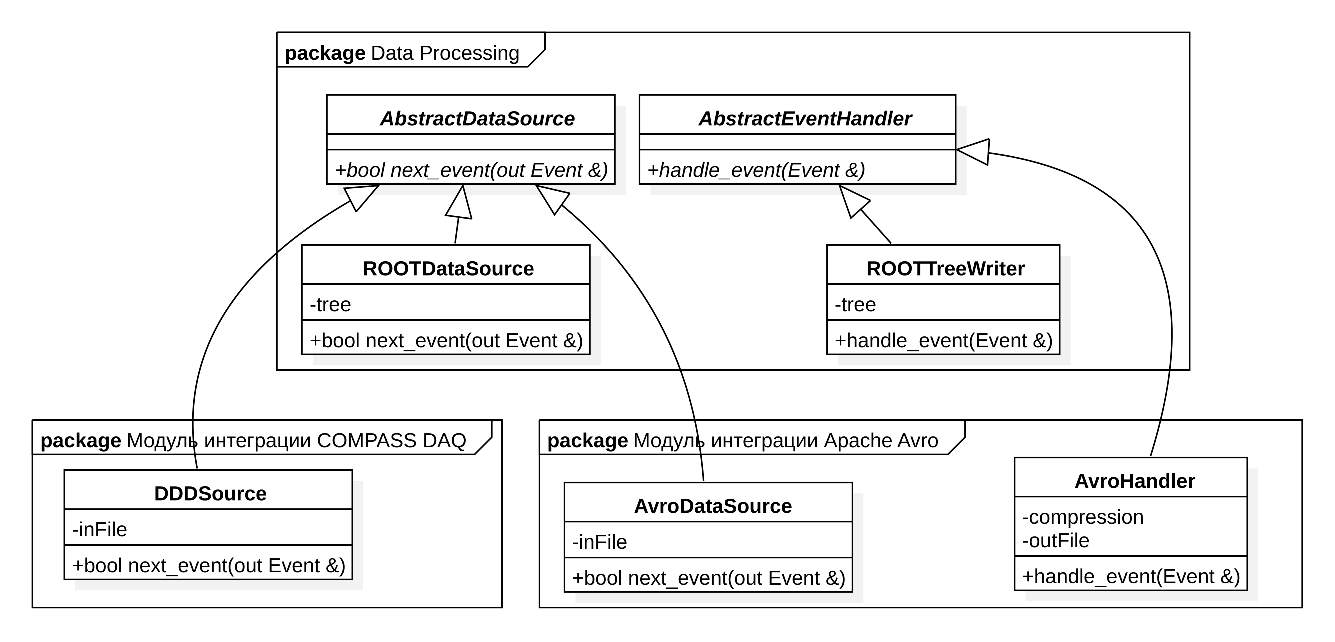
\includegraphics[width=0.95\linewidth]{images/illustrative/data-sources-example.eps}
    \caption{Диаграмма классов иллюстрирующая отношения классов реализующих различные форматы хранения событий}
    \label{fig:data-sources-example}
\end{figure}

Как и в случае с объектной моделью события, рассмотренной ранее,
автоматическая генерация декодировщиков данных относится преимущественно
к внутренним протоколам программного окружения. Интеграция с внешними
источниками осуществляется через отдельные модули, поддерживаемые вручную.

Так, в частности, важнейшим источником является декодирование данных,
считанных напрямую из системы сбора данных (DAQ), которое опирается
на библиотеку кодирования COMPASS~\cite{compass-daq}.

Таким образом, модуль реализующий интерфейс источника данных обычно
является промежуточным слоем между библиотекой и ядром системы.

\subsection{Иерархия детекторов в выходных данных}

Класс \texttt{TDirAdapter} (из окружения ROOT) предоставляет
часто используемые операции при отображении множества детекторов в связанный
набор экземпляров подкласса \texttt{TObject} допускающих
хранение внутри \texttt{TDirectory}. В таком виде удобно
размещать большие наборы гистограмм и
графиков соответствующих индивидуальным детекторам в рамках одного
обработчика. Так, например, с применением идентификаторов детектора,
наглядную иерархию объектов отвечающую
логической структуре детектора изображённую на
рисунке~\ref{fig:tobject-hierarchy} можно получить подстановкой
семнтических элементов идентификатора в простой текстовый шаблон.

\begin{figure}
    \centering
    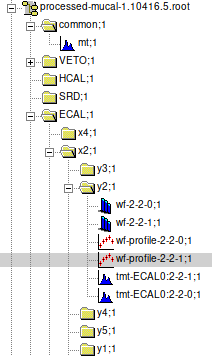
\includegraphics[width=0.25\linewidth]{images//illustrative/items-structure-in-root-file.png}
    \caption{Иерархия объектов внутри \texttt{TFile} порождаемая
    идентификатором детектора на основе шаблонных путей}
    \label{fig:tobject-hierarchy}
\end{figure}

Обработчики включающие \texttt{TDirAdapter} обычно
предусматривают переопределение шаблонов путей для адаптации к
конкретным пользовательским приложениям в тех случаях когда
спецификация входного файла каким-то образом ограничена.

\subsection{Извлечение характеристик распределений}

Например, часто возникающая практическая задача отыскания
коэффициентов распределений на основе особенностей различных
спектров может быть обусловлена в виде короткого конфигурационного
файла задающего:
\begin{itemize}
    \item Шаблон имени гистограммы при помощи регулярных
    выражений с именованными группами захвата для извлечения
    имени детектора и индекса элемента,
    \item Обозначения особенности на
    спектре -- например <<первый минимум по порядку>>,
    <<второй максимум по высоте>>.
\end{itemize}

\begin{figure}
    \centering
    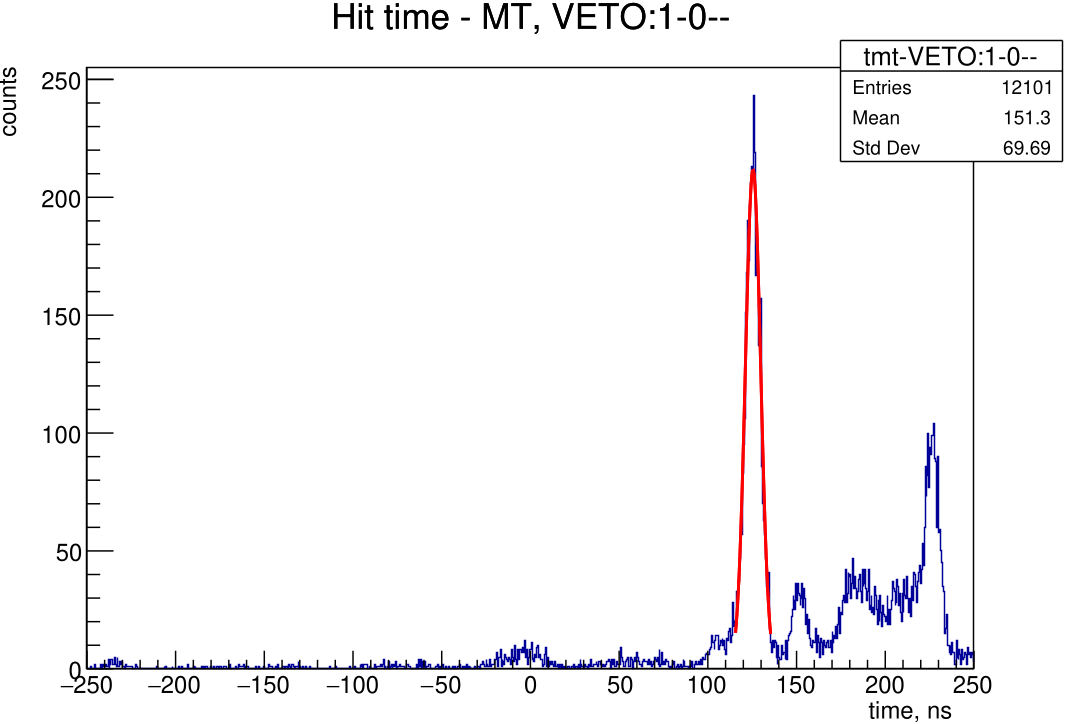
\includegraphics[width=0.5\linewidth]{images//illustrative/tmt-fit-example.png}
    \caption{Пример автоматического выделения основного пика во временном
    распределении мюонного сигнала в вето-детекторе}
    \label{fig:placeholder}
\end{figure}

Обобщение практики применения таких процедур показывает, что количество
особенностей сравнительно невелико, и в большинстве случаев логика,
необходимая для калибровки или автоматизированного анализа, может быть
задана в виде компактной спецификации.

\section{Визуализация событий}

\begin{figure}
    \centering
    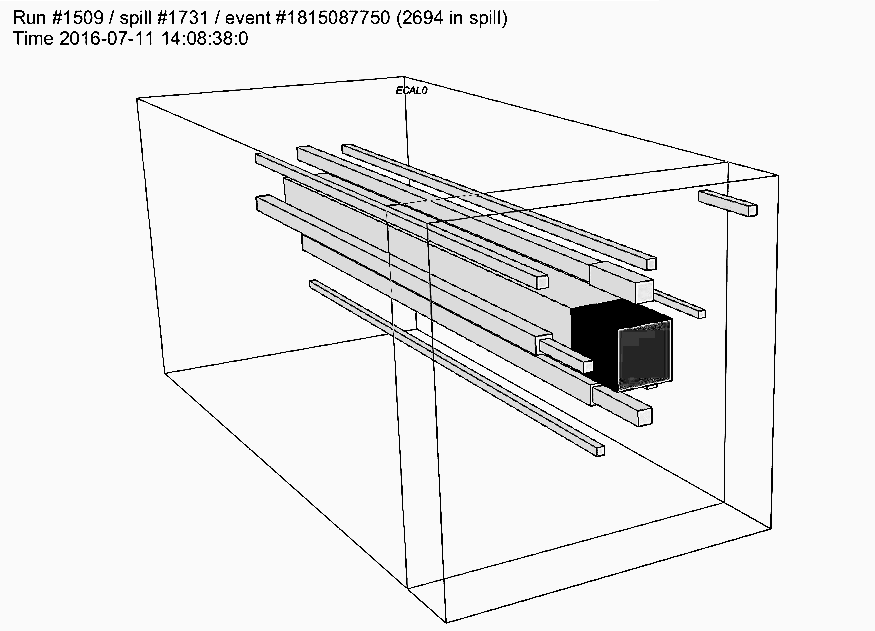
\includegraphics[width=0.5\linewidth]{images//illustrative/ecal-evidplay-example-3d.png}
    \caption{Визуализация события в ECAL}
    \label{fig:event-display-ecal-only}
\end{figure}

\begin{figure}
    \centering
    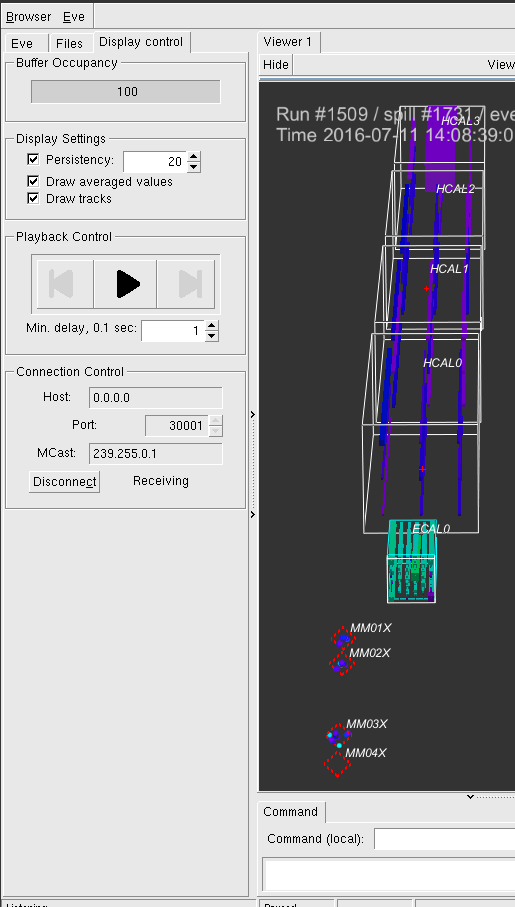
\includegraphics[width=0.25\linewidth]{images//illustrative/event-display-mult.png}
    \caption{Общий вид приложения}
    \label{fig:event-display-3d}
\end{figure}
